%%%%%%%%%%%%%%%%%%%%%%%%%%%%%%%%%%%%%%%%%%%%%%%%%%%%%%%%%%%%%%%%%%%%%%%%
%    INSTITUTE OF PHYSICS PUBLISHING                                   %
%                                                                      %
%   `Preparing an article for publication in an Institute of Physics   %
%    Publishing journal using LaTeX'                                   %
%                                                                      %
%    LaTeX source code `ioplau2e.tex' used to generate `author         %
%    guidelines', the documentation explaining and demonstrating use   %
%    of the Institute of Physics Publishing LaTeX preprint files       %
%    `iopart.cls, iopart12.clo and iopart10.clo'.                      %
%                                                                      %
%    `ioplau2e.tex' itself uses LaTeX with `iopart.cls'                %
%                                                                      %
%%%%%%%%%%%%%%%%%%%%%%%%%%%%%%%%%%
%
%
% First we have a character check
%
% ! exclamation mark    " double quote  
% # hash                ` opening quote (grave)
% & ampersand           ' closing quote (acute)
% $ dollar              % percent       
% ( open parenthesis    ) close paren.  
% - hyphen              = equals sign
% | vertical bar        ~ tilde         
% @ at sign             _ underscore
% { open curly brace    } close curly   
% [ open square         ] close square bracket
% + plus sign           ; semi-colon    
% * asterisk            : colon
% < open angle bracket  > close angle   
% , comma               . full stop
% ? question mark       / forward slash 
% \ backslash           ^ circumflex
%
% ABCDEFGHIJKLMNOPQRSTUVWXYZ 
% abcdefghijklmnopqrstuvwxyz 
% 1234567890
%
%%%%%%%%%%%%%%%%%%%%%%%%%%%%%%%%%%%%%%%%%%%%%%%%%%%%%%%%%%%%%%%%%%%
%

\documentclass[12pt]{iopart}
\usepackage{multirow}
\usepackage[dvipsnames]{xcolor}
\usepackage{graphicx}
\usepackage[sorting=none]{biblatex} %Imports biblatex package
\addbibresource{references.bib} %Import the bibliography file
\newcommand{\gguide}{{\it Preparing graphics for IOP Publishing journals}}
%Uncomment next line if AMS fonts required
%\usepackage{iopams}  
\graphicspath{{Figures/}}

\begin{document}

\title{Using Machine Learning to predict the behavior of moderate pressure capacitively coupled plasmas}
%JMP is a specific bit of software that is used to do designed experiments - and similar studies. That is NOT new. What is important here is the ML bit.
\author{Shadhin Hussain,$^{ a}$ David J. Lary,$^{ a}$ Ken Hara,$^{b}$ Kallol Bera,$^{c}$ Shahid Rauf,$^{c}$  Matthew Goeckner$^a$}

\address{$^a$Department of Physics, University of Texas at Dallas, Richardson TX, 75080 \\
$^b$Aeronautics and Astronautics, Stanford University,  Stanford CA, 94305 \\
$^c$Applied Materials Corp, Santa Clara, CA 95054}
\ead{Shadhin.Hussain@utdallas.edu, david.lary@utdallas.edu, \\ kenhara@stanford.edu, Kallol\_Bera@amat.com, Shahid\_Rauf@amat.com, goeckner@utdallas.edu}
\vspace{10pt}
\begin{indented}
\item[]February 2023
\end{indented}

\begin{abstract}
\textcolor{red}{One two three... need to write this.}
\end{abstract}

%
% Uncomment for keywords
%\vspace{2pc}
%\noindent{\it Keywords}: XXXXXX, YYYYYYYY, ZZZZZZZZZ
%
% Uncomment for Submitted to journal title message
%\submitto{\JPA}
%
% Uncomment if a separate title page is required
%\maketitle
% 
% For two-column output uncomment the next line and choose [10pt] rather than [12pt] in the \documentclass declaration
%\ioptwocol
%



\section{Introduction}
Laboratory plasmas, particularly those used in the semiconductor industry,  are complex environments that are influenced by many external `control parameters'.[REF] These control parameters include: external power (power deposition method, power level, supplied power frequency); neutral gas (species, pressure, flow rate); chamber geometry/materials.  Understanding fundamental physical phenomena such as collision, diffusion, particle and energy balance, and gas chemistry is essential to comprehending the processes that govern plasma dynamics at different conditions.  Under some conditions, it is possible to deploy a large suite of diagnostics and via those results develop effective models of the plasma system.  Under other conditions, such as intermediate or high pressures, traditional diagnostics (Langmuir probes, etc) will not function correctly and detailed models of the plasmas are harder to develop.  

Capacitively coupled plasmas (CCPs) are one of the most commonly used laboratory plasmas, due to their wide use in the semiconductor industry.  CCPs are commonly classified by their operating pressure and the resulting ``heating mode.'' [NEEDS REF] A low-pressure discharge is typically considered to be within the range of tens of µTorr up to tens of mTorr, while the moderate/intermediate pressure regime spans from 1-100 Torr.[NEEDS REF] These two pressure regimes differ significantly in terms of breakdown, heating, and maintaining the discharge.[NEEDS REF] Although the general pressure dependence of CCPs is known, studies of these systems in the intermediate pressure regime are limited.  This is in part because `traditional' diagnostic tools, such as Langmuir Probes, do not work at these intermediate pressures.[NEEDS REF]  None-the-less, such intermediate pressure CCP systems are widely utilized in industrial applications, including carbon nanotube and diamond-like carbon deposition processes, flat panel display and solar panel fabrication industries, as well as an active medium for CO$_2$ lasers. However, despite their widespread use, a lack of understanding of radio frequency (RF) CCP discharges in these pressure ranges has resulted in most designs being based on empirical studies.

For many years, researchers deploying plasma systems in the semiconductor industry made use of Design of Experiment (DOE) studies to ascertain control parameter regimes which would result in effective processing of a wafer.   Specifically... NEED some references [REFS] to DOE studies and narrowing in on the `correct parameters' needed in a given process.   Need a description of how DOE studies are set up.  DOE studies do not allow one to build models of a process - just find which combination of parameters will give rise to `proper' processing of a wafer.

Modeling and forecasting the dynamics of complex systems such as intermediate pressure CCP systems remains a challenge due to the interactions of physical and chemical processes across multiple scales. Observational data, including multi-fidelity data from sensors, can provide valuable insights, but integrating it into existing models is difficult. On the other hand, Machine Learning (ML) approaches, particularly deep learning, can extract features from massive amounts of data, but may lack interpretability and physical consistency.


More recently, traditional DOE studies have begun to be replaced by Machine Learning (ML) studies.  ML holds the potential to expand our understanding of laboratory plasmas operating under conditions that are largely unexplored.[NEEDS REF]  Early results with ML already show promise in bridging this gap. [NEEDS REF] ML allows us to \textit{learn by example}, and to \textit{give our data a voice}. It is especially useful for applications for which we do \textit{not} have a complete theory but the trends are of interest to us. Machine learning is an automated implementation of the scientific method \cite{Domingos:2015}, following the same process of generating, testing and discarding or refining hypotheses. While a researcher may spend their entire career coming up with and testing a few hundred hypotheses, a machine-learning system can do the same in a fraction of a second. Machine learning provides an objective set of tools for automating discovery. It is therefore not surprising that machine learning is currently revolutionizing many areas of science, technology, business and medicine \cite{Lary:2016}.

In this article, we will examine the use of ML to predict trends in moderate pressure CCPs.  Here, we make use of a  Design of Experiment (DOE)  organized experimental study of the current-voltage (I-V) signal in the deposited power. We will explore the efficacy of various ML models on the resultant I-V data sets in predicting I-V data under other conditions. We will show results and compare the prediction accuracy of different ML models including supervised regression as well as supervised classification approaches, as well as of least square fitting using a common DOE software tool (JMP).

In section \ref{Sect:ExpSetup} we will describe the experimental system and related diagnostic tools.  This will include a review of how the measured data is analyzed to arrive at our database.  In section \ref{Sect:Database} we will present the resultant data that will be used in the our ML study. In section 
\ref{Sect:RegressionAnalysis} we will deploy four common ML regression analysis models to examine our experimental data.  In section \ref{Sect:Classification} we will explore ML classification models with our experimental data. Finally we provide our conclusions in section \ref{Sect:Conclusions}.

\section{Experimental setup}\label{Sect:ExpSetup}
\textcolor{black}{The experiments in this study were conducted inside the modified Gaseous Electronics Chamber (mGEC) [20, 21, 22, 23, 24]. The mGEC reactor's design has been discussed in detail by Goeckner et al. [20]. Originally, the mGEC had an inductively coupled plasma (ICP) source, which was later converted into a capacitively coupled plasma (CCP) source [21]. A general schematic of the CCP system is depicted in Figure 1. The plasma-facing powered and grounded aluminum electrodes are surrounded by grounded electrode shields, maintaining a gap of about 2.5 mm between the electrode and shield. The powered electrode measures 11.4 cm in diameter, while the grounded electrode is 15 cm in diameter. The gap between them is adjustable from 2 cm to 12.5 cm. Although the mGEC has internal walls to control chamber diameter, they were not utilized in these studies.}

\textcolor{black}{An rf signal generator (Keysight 33600 A Waveform generator) produced a \hbox{13.56 MHz} signal, amplified by an ENI A-300 rf Power Amplifier to create input power. Baseline measurements of supplied and reflected power were taken with a Bird Model 43 wattmeter. The power then passed through an L-type match network, equipped with two adjustable capacitors which were set to minimize the reflected power, before reaching the powered electrode. The load encompassed the plasma, DC bias circuit, current and voltage probes (I-V), the powered electrode, the 50-ohm transmission line, and the grounded chamber with a grounded electrode/chuck.}

\textcolor{black}{As is shown in Figiure \ref{Fig:mGEC}, the DC self-bias, current, and voltage were measured on the 50-ohm transmission line between the match network and powered electrode. The DC self-bias measurement setup featured an 84 µH choke followed by a capacitor to ground for measuring bias. The current probe utilized a Rogowski coil (Pearson electronics 2877), while the voltage probe was built in-lab by capacitively coupling the transmission line's powered lead through Teflon. An identical Rogowski coil measured current through the grounded electrode. High-speed data acquisition was performed using a Teledyne Lecroy HDO 6104B oscilloscope with 12-bit vertical resolution and $10^{10}$ samples per second. To enhance voltage probe sensitivity to plasma sheath harmonics, it was connected to the oscilloscope's 50-ohm input. A fast Fourier transform (FFT) analysis discerned fundamental and higher harmonics within waveforms, crucial for power and impedance calculations of the sheath and plasma bulk.}

\begin{figure}[ht!]
\begin{center}
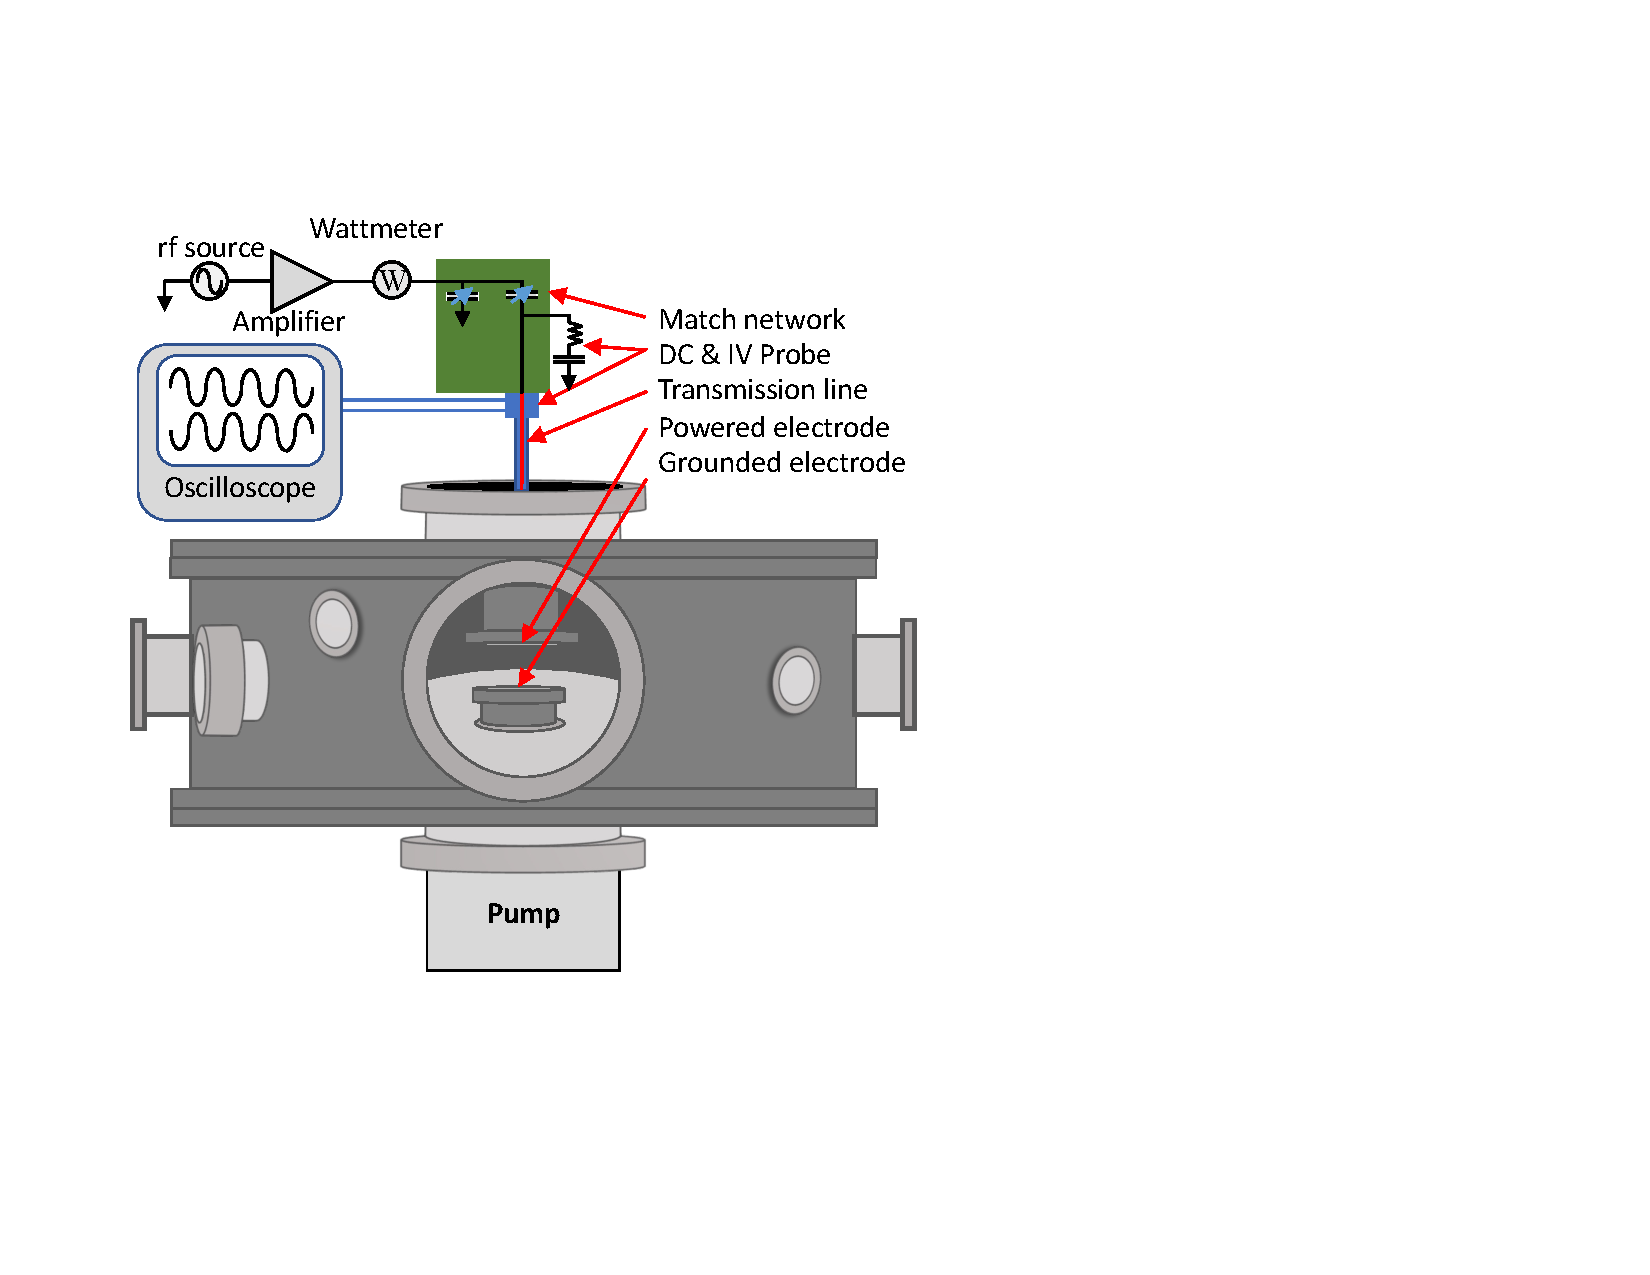
\includegraphics[width=.89\textwidth]{mGEC.pdf}
	\caption{A sketch of the modified Gaseous Electronics Conference (mGEC) reference cell\cite{goeckner2004modified}.}
	\label{Fig:mGEC}
\end{center}
\end{figure}

\textcolor{black}{Calibrating both current and voltage probes involved obtaining amplitude and phase factors as functions of frequency, including relative phase. Oscilloscope's 50-ohm input provided a known resistive load for probe calibration. Calculating I-V magnitude and phase at the electrode relied on FFT data from the probes and the parasitic impedances listed in Table \ref{tab:Measured_impedance}. The electrical length of the transmission line between probe and electrode, as measured by a network analyzer, was accounted for when reconstructing the I-V waveform at the powered electrode. Additionally, an equivalent circuit, see Figure \ref{Fig:mGEC_Circuit}, incorporating measured parasitics, Table \ref{tab:Measured_impedance}, was used to calculate current and voltage at the electrodes from raw data at the probes. The methods of parasitic impedance, delay measurements, and calibration are described by Press \cite{press2019sub}. Typical measured and reconstructed I-V traces are shown in \ref{Fig:Current_v_time}.}

\begin{figure}[ht!]
\begin{center}
\includegraphics[width=.99\textwidth]{mGEC_Circuit.pdf}
	\caption{Circuit elements of the I-V measurement experiment. Measured parasitic impedances at $Z_1$, $Z_2$,$Z_{g1}$, and $Z_{g2}$ are given in Table \ref{tab:Measured_impedance}.} 
	\label{Fig:mGEC_Circuit}
\end{center}
\end{figure}

\begin{table}[]
    \centering
    \begin{tabular}{|c|c|c|c|c|}
        \hline
        Frequency (MHz) & $Z_1 (\Omega)$ & $Z_2 (\Omega)$ & $Z_{g1} (\Omega)$ & $Z_{g2} (\Omega)$ \\
        \hline
        13.56 & 28.97i & 4.96-113.87i & 1.1+11.95i & -71.79i\\
        27.12 & 0.12+7.6i & 2.39-18.68i & 1.1+23.91i & -35.89i \\
        40.68 & 11.48+81.83i & 2.52+35.96i & 1.1+35.86i & -23.93i \\
        \hline
    \end{tabular}
    \caption{Measured parasitic impedances $Z_1$, $Z_2$, $Z_{g1}$, and $Z_{g2}$.  These values were used to determine the currents and voltages at the electrode faces from the measured values. \textbf{Cite your first paper.}}
    \label{tab:Measured_impedance}
\end{table}

\begin{figure}[ht!]
\begin{center}
\begin{minipage}{0.495\textwidth}
    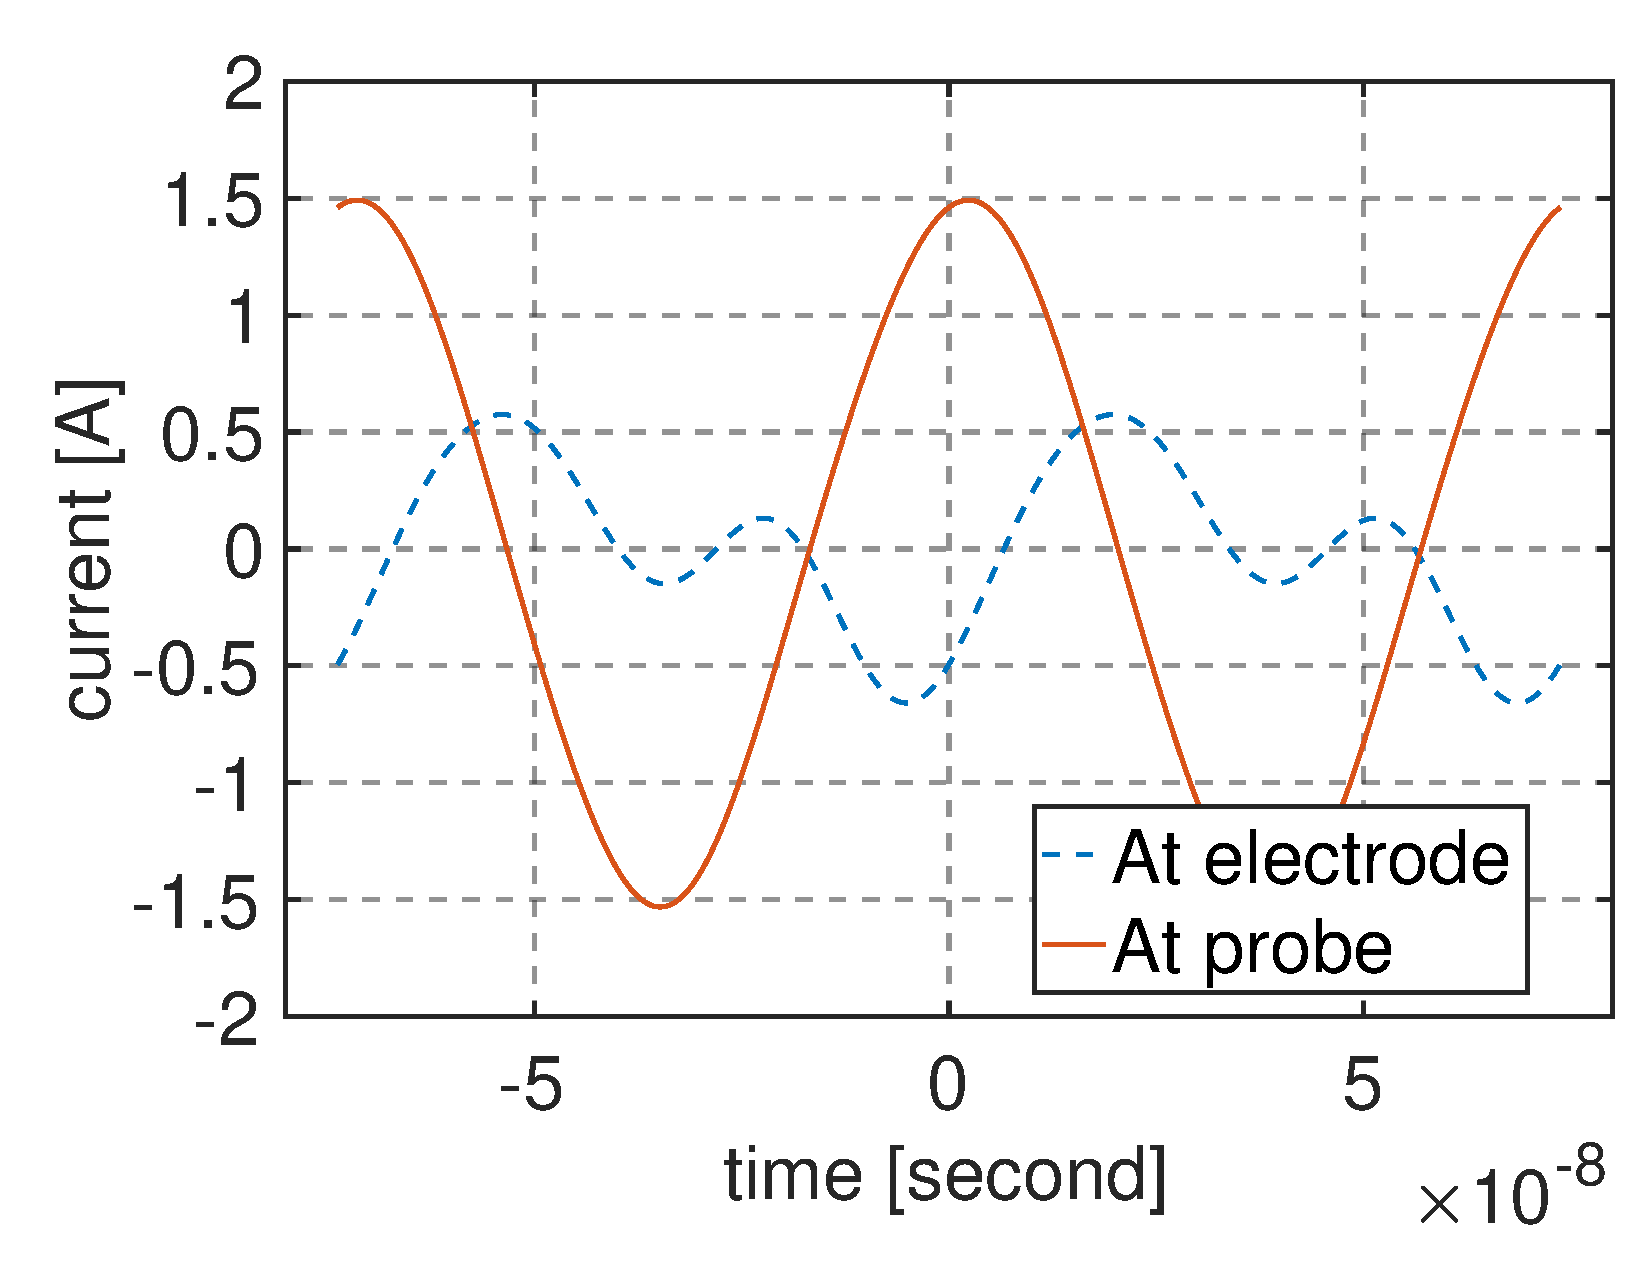
\includegraphics[width=1\textwidth]{electrode_vs_probe_current.pdf}
\end{minipage}
\begin{minipage}{0.495\textwidth}
    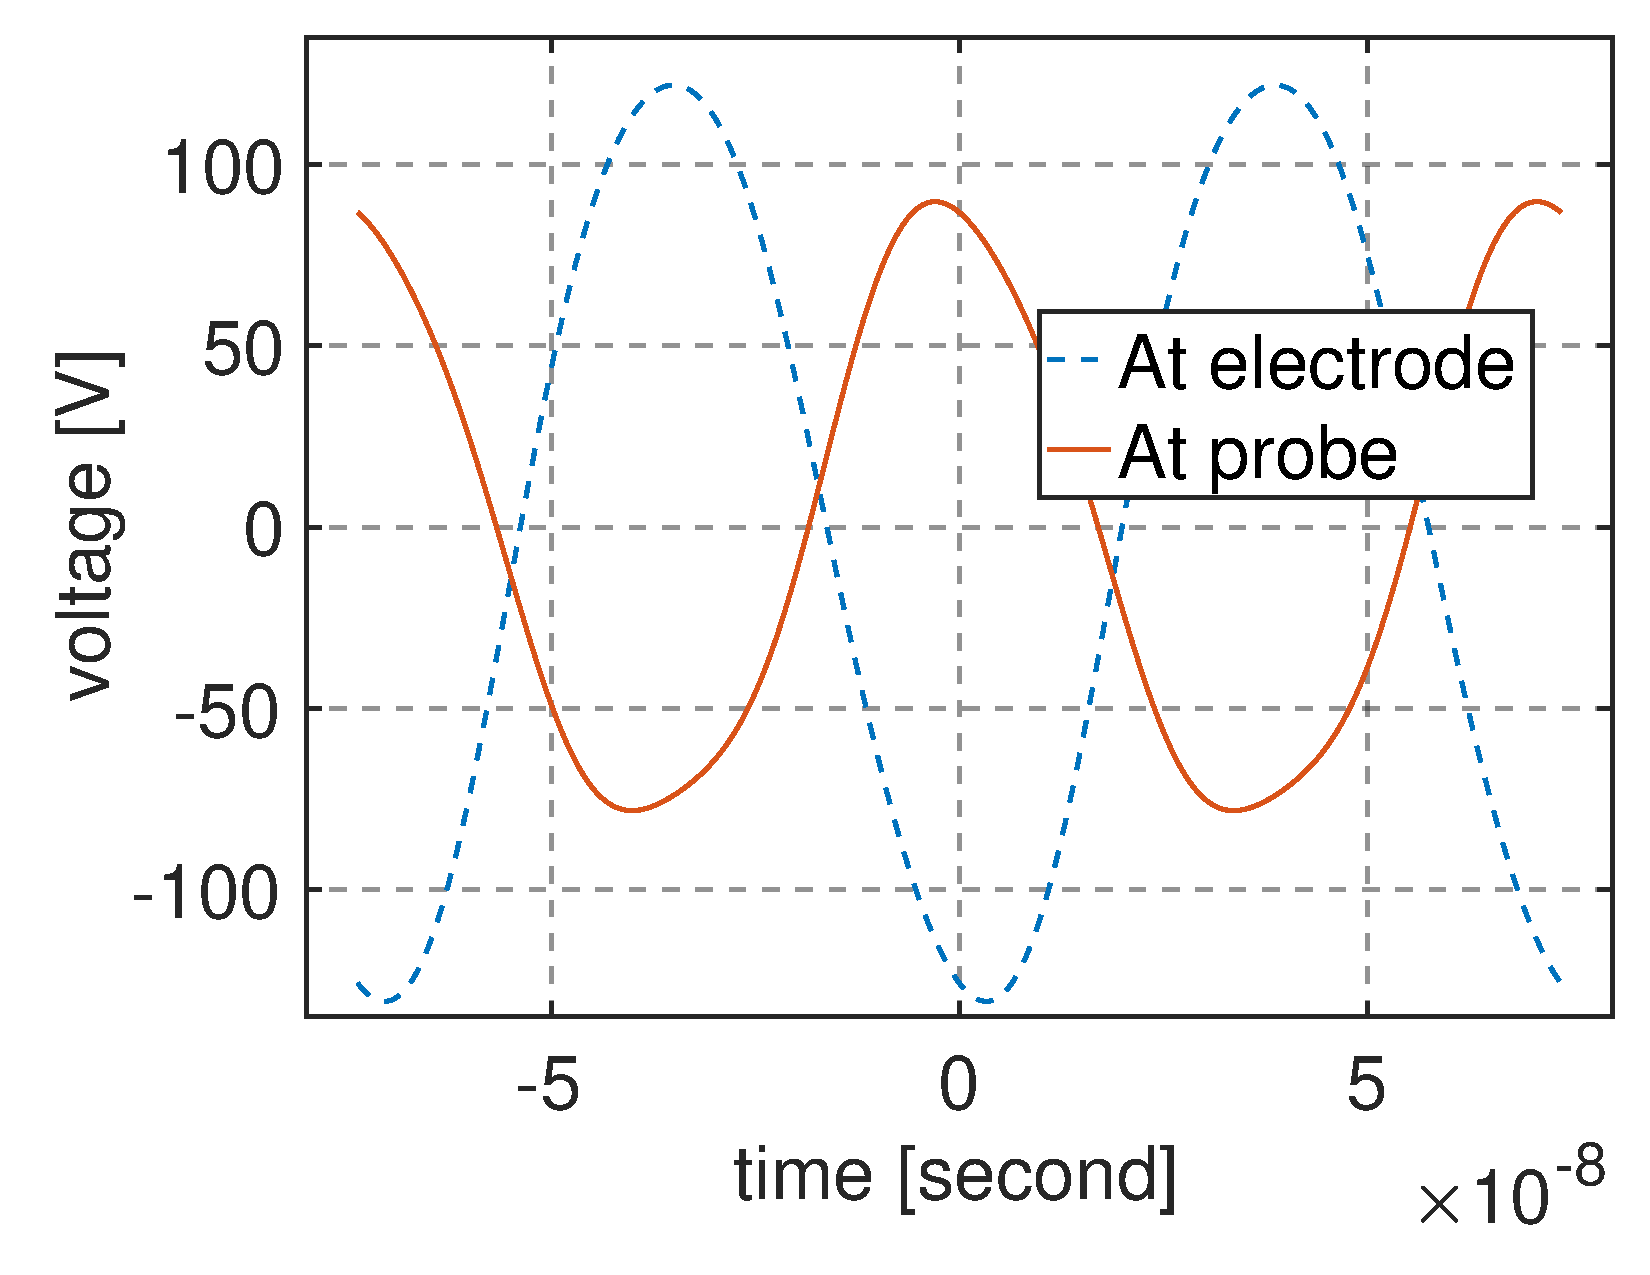
\includegraphics[width=1\textwidth]{electrode_vs_probe_voltage.pdf}
\end{minipage}
	\caption{Example (left) rf current (right) rf voltage traces measured at the probe and reconstructed at the electrode by correcting for parasitic impedances and transmission delay for a 0.5 Torr argon discharge. \textbf{Needs to reference the first paper.}}
	\label{Fig:Current_v_time}
\end{center}
\end{figure}

\textcolor{black}{Both electrodes' currents comprise conductive and displacement components. Conductive current originates from the faster-moving electrons, capable of tracking rapid potential shifts induced by the RF field due to their lighter mass compared to ions. As electrons exhibit a roughly Maxwellian velocity distribution, the electron density at the electrode and electron current ($i_e$) adhere to the Boltzmann relation. This leads to an exponential decline in electron density and current as potential drops below the plasma potential in the sheath \cite{sobolewski1995electrical},}
\begin{equation} 
    i_e=i_k\exp[e\phi\left(t\right)/k_B T_e],
    \label{eqn:electron conduction}
\end{equation}
where $T_e$ is the electron temperature, $k_B$ is Boltzmann's constant. $i_k$ is a function of bulk electron density and temperature \cite{sobolewski1995electrical} and
\begin{equation} 
    \phi\left(t\right) = -\phi_{dc} + \phi_1\cos(\omega t).
    \label{eqn:sheath voltage}
\end{equation}
is the voltage across the sheath.  In this context, $\phi_{dc}$ represents the DC voltage, and $\phi_1\cos(\omega t)$ signifies the fluctuating voltage across the sheath – part of it being the RF voltage applied. Electrons react to the dynamic field, while ions are influenced solely by the average potential. Consequently, a predominantly DC current $i_{ion}$ arises from ions, dictated by electrode area $A$, ion density $n_i(x)$, and velocity $u_i(x)$ at distance $x$ from the powered electrode \cite{sobolewski1995electrical},
\begin{equation} 
    i_{ion}=e\ n_i\left(x\right)u_i\left(x\right)\ A 
\end{equation} 
Thus, the total conduction current $i_c\left(t\right)$ is given by, 
\begin{equation}
i_c\left(t\right)=i_k\exp[e\phi\left(t\right)/k_BT_e]+i_{ion}
\label{eqn:conduction_current}
\end{equation}
Likewise, displacement current stems from the varying sheath electric field. By exploiting the property that the derivative of an even sinusoidal function is odd, one can dissect the overall current into its conductive and displacement constituents \cite{sobolewski1995electrical}. This observation becomes apparent when considering the definition of displacement current, 
\begin{eqnarray}
    i_d\left(t\right) &=\epsilon_0A\frac{d}{dt}[\phi \left(t\right)/ s\left(t\right)] \\
    &=\frac{\epsilon_0A} {s\left(t\right)}\frac{d\phi \left(t\right)}{dt}-\phi \left(t\right)\frac{\epsilon_0A}{s\left(t\right)^2}\frac{d}{dt}s\left(t\right)
\label{eqn:displacement_current}
\end{eqnarray}
Here, with $s\left(t\right)$ as the sheath thickness and $A$ as the electrode's surface area, if $\phi\left(t\right)$ takes the form of an even sinusoidal function, $i_c$ is also even, while $i_d$ is odd, assuming that the sheath thickness is synchronized with the applied voltage \cite{panagopoulos1999plasma}. 

\begin{table}[]
    \centering
%    \begin{tabular}{|c|c|c|}
\begin{tabular}{|p{1cm}|p{2cm}|p{12.5cm}|}
        \multicolumn{3}{l}{Measured} \\ 
        \hline
        & Variable & Description\\ 
        \hline 
        1 & $V_{DC}$ & DC self-bias\\
        2 & $V_{rf,1}$ & Total 1st harmonic peak to peak voltage\\
        3 & $V_{rf,2}$ & Total 2nd harmonic peak to peak voltage\\
        4 & $V_{rf,3}$ & Total 3rd harmonic peak to peak voltage\\
        5 & $I_{rf,1}$ & Total driven electrode peak to peak current (1st harmonic)\\
        6 & $I_{rf,2}$ & Total driven electrode peak to peak current (2nd harmonic)\\
        7 & $I_{rf,3}$ & Total driven electrode peak to peak current (3rd harmonic)\\
        8 & $I_{gnd,1}$ & Total ground electrode peak to peak current (1st harmonic)\\
        9 & $I_{gnd,2}$ & Total ground electrode peak to peak current (2nd harmonic)\\
        10 & $I_{gnd,3}$ & Total ground electrode peak to peak current (3rd harmonic)\\
        11* & $\nu_{1,p}$ & Phase difference at the probe (1st harmonic) \\
        12 & $\nu_{2,p}$ & Phase difference at the probe (2nd harmonic) \\
        13 & $\nu_{3,p}$ & Phase difference at the probe (3rd harmonic) \\
        \hline \multicolumn{3}{l}{Calculated} \\ \hline
        & Variable & Description\\ 
        \hline 
        14* & $I_{cond,1}$ & Driven electrode peak to peak conduction current (1st harmonic) \\
        15 & $I_{cond,2}$ & Driven electrode peak to peak conduction current (2nd harmonic) \\
        16 & $I_{cond,3}$ & Driven electrode peak to peak conduction current (3rd harmonic) \\       
        17* & $I_{disp,1}$ & Driven electrode peak to peak displacement current (1st harmonic) \\     
        18 & $I_{disp,2}$ & Driven electrode peak to peak displacement current (2nd harmonic) \\
        19 & $I_{disp,3}$ & Driven electrode peak to peak displacement current (3rd harmonic) \\
        20* & $R_{1}$ & Resistive impedance at the driven electrode (1st harmonic) \\
        21 & $R_{2}$ & Resistive impedance at the driven electrode (2nd harmonic) \\
        22 & $R_{3}$ & Resistive impedance at the driven electrode (3rd harmonic) \\
        23* & $X_{1}$ & Reactive impedance at the driven electrode (1st harmonic) \\
        24 & $X_{2}$ & Reactive impedance at the driven electrode (2nd harmonic) \\
        25 & $X_{3}$ & Reactive impedance at the driven electrode (3rd harmonic) \\
        26* & $P_{1,e}$ & Average power at the driven electrode (1st harmonic) \\
        27 & $P_{2,e}$ & Average power at the driven electrode (2nd harmonic) \\      
        28 & $P_{3,e}$ & Average power at the driven electrode (3rd harmonic) \\
        29* & $P_{1,p}$ & Average power at the probe (1st harmonic) \\
        30 & $P_{2,p}$ & Average power at the probe (2nd harmonic) \\
        31 & $P_{3,p}$ & Average power at the probe (3rd harmonic) \\
        32* & $\nu_{1,e}$ & Phase difference at the driven electrode (1st harmonic) \\
        33 & $\nu_{2,e}$ & Phase difference at the driven electrode (2nd harmonic) \\
        34 & $\nu_{3,e}$ & Phase difference at the driven electrode (3rd harmonic) \\
\hline
    \end{tabular}
    \caption{The 34 directly measured and calculated parameters in this study.  Parameters denoted with a `*' are those that are affected by $\nu_{1,e}$, the 1st harmonic phase difference at the driven electrode.  Others are independent of that phase. \textcolor{red}{\textbf{Should we eliminate the `*'?}}}
    \label{tab:Measured_parameters}
\end{table}

\section{mGEC moderate pressure plasma Database}\label{Sect:Database}

A study of intermediate pressure plasma can consist of an indefinite number of experiments involving many adjustable control parameters, such as feed gas, power, pressure, interelectrode gap, etc. To understand the effects of these control parameters, current and voltages (I-V) were measured at combinations of four control parameters: applied power (10-70 W), electrode gap (20-28 mm), operating pressure (0.5-2.5 Torr), and ratios of feed gases ($Ar/N_2$, $Ar/O_2$, $N_2/O_2$). The specific combinations of these parameters were determined using a commercial software package (JMP). The order in which the runs were taken was randomized. The experiments were repeated four times, allowing for either the direct measurement or calculation of the parameters shown in Table \ref{tab:Measured_parameters}. The primary I-V quantities were plotted against each control parameter and p-values, see Table \ref{tab:DOE_Results}, were calculated to compare the fit between the control and measured parameters using JMP. Variation in electrode gap was found to have an insignificant correlation with all the measured quantities and thus was kept fixed at 24 mm for subsequent experiments.  

\begin{table}[]
    \centering
   \begin{tabular}{|c|c|c|c|c|c|c|}
        \hline
        \begin{minipage}{0.15\textwidth}\begin{center}
             Control \\ Parameter \end{center} \end{minipage} & \begin{minipage}{0.1\textwidth}\begin{center}
             Ar flow \\ (\%) \end{center} \end{minipage} & \begin{minipage}{0.1\textwidth}\begin{center}
             $N_2$ flow \\ (\%) \end{center} \end{minipage}  & \begin{minipage}{0.1\textwidth}\begin{center}
             $O_2$ flow \\ (\%) \end{center} \end{minipage} & \begin{minipage}{0.1\textwidth}\begin{center}
             Pressure \\ (Torr) \end{center} \end{minipage} & \begin{minipage}{0.1\textwidth}\begin{center}
             Gap \\ (mm) \end{center} \end{minipage} & \begin{minipage}{0.1\textwidth}\begin{center}
             Power \\ (Watts) \end{center} \end{minipage} \\
        \hline
        \multicolumn{7}{l}{Powered electrode} \\
        \hline
        $V_{DC}$ & 0.0024 & 0.0311 & 0.4070 & $<$0.0001 & 0.7025 & $<$0.0001\\
        $V_{rf,1}$ & 0.0012 & 0.0043 & 0.7295 & 0.0252 & 0.7869 & $<$0.0001\\
        $V_{rf,2}$ & 0.0001 & 0.0444 & 0.0971 & 0.0007 & 0.9940 & $<$0.0001\\
        $V_{rf,3}$ & 0.9278 & 0.8050 & 0.8758 & $<$0.0001 & 0.8299 & $<$0.0001\\
        $I_{rf,1}$ &  $<$0.0001 & 0.0083 & 0.0911 & 0.9634 & 0.8046 & $<$0.0001\\
        $I_{rf,2}$ & 0.0001 & 0.0450 & 0.0970 & 0.0007 & 0.9933 & $<$0.0001\\
        $I_{rf,3}$ & 0.8136 & 0.7093 & 0.8912 & $<$0.0001 & 0.8446 & $<$0.0001\\
        \hline
        \multicolumn{7}{l}{Ground electrode} \\
        \hline
        $I_{gnd,1}$ & 0.0009 & 0.0225 & 0.3313 & 0.0031 & 0.1812 & $<$0.0001\\
        $I_{gnd,2}$ & 0.3328 & 0.4769 & 0.7984 & $<$0.0001 & 0.3369 & $<$0.0001\\
        $I_{gnd,3}$ & 0.0585 & 0.1756 & 0.5999 & 0.0012 & 0.5578 & $<$0.0001\\
        \hline
    \end{tabular}
    \caption{p-values for control parameter effects on measured current and voltages.  It is noted that the observed p-value for gap is always large, indicating that the gap, over the range studied, is not important in the results. In light of this, the gap was not examined in much of the additional parameter sweeps.}
    \label{tab:DOE_Results}
\end{table}


 Once the screening was completed, comprehensive experiments were conducted across power, pressure and gas mixtures. Experiments were run for all combinations of pressure of 0.5, 1.5, 2.5 Torr, and nominal power of 10, 25, 40, 55, 70 Watts (read from the wattmeter) for pure argon, nitrogen, and oxygen as well different mixtures between them. See Table \ref{tab:Datasets}. Each experiment was run for a total of four times and 13 full RF cycles were processed for each run. Each cycle consisted of about 738 data points acquired by the oscilloscope, giving a phase resolution of about one-half degree. A 13x4 matrix was built for all parameters of interest for each run. For each of the four iterations, average parameter values were calculated from the set of 13 acquired cycles. To study interpolation using machine learning, additional data were later collected at 1 Torr and 2 Torr for the same gap, gas mixtures and power ranges. Data at 1 and 2 Torr were collected only once and post-processed in a similar way.
\begin{table}[]
    \centering
    \begin{tabular}{|c|c|c|c|c|c|c|c|}
        \hline
            Data set & Factorial & \# of runs & \begin{minipage}{0.08\textwidth} Mixture \end{minipage} & \begin{minipage}{0.08\textwidth}\begin{center}
            \vspace{0.2cm} Flow ratio \\ (\%) \vspace{0.2cm} \end{center} \end{minipage} & \begin{minipage}{0.08\textwidth}\begin{center}
            Pressure \\ (Torr) \end{center} \end{minipage}  & \begin{minipage}{0.08\textwidth}\begin{center}
            Power \\ (W) \end{center} \end{minipage} & \begin{minipage}{0.08\textwidth}\begin{center}
            Gap \\ (mm) \end{center} \end{minipage}  \\
        \hline
        1 & level 2 & 4 &
        \begin{minipage}{0.07\textwidth}\begin{center}
             $Ar$:$O_2$ \\ $Ar$:$N_2$ \\ $N_2$:$O_2$
            \end{center}
        \end{minipage} & 
        \begin{minipage}{0.1\textwidth}\begin{center}
              0:100 \\ 33:67 \\ 67:33 \\ 100:0
        \end{center}\end{minipage} & 
        \begin{minipage}{0.1\textwidth}\begin{center}
              0.5 \\ 1.5 \\ 2.5
        \end{center}\end{minipage}  & 
        \begin{minipage}{0.1\textwidth}\begin{center}
             \vspace{0.2cm} 10 \\ 25 \\ 40 \\ 55 \\ 70 \vspace{0.2cm}
        \end{center}\end{minipage} & 
        \begin{minipage}{0.1\textwidth}\begin{center}
              20 \\ 24 \\ 28
        \end{center}\end{minipage} \\
        \hline
        2 & Full & 4 & \begin{minipage}{0.15\textwidth}\begin{center}
             $Ar$:$O_2$ \\ $Ar$:$N_2$ \\ $N_2$:$O_2$
            \end{center}
        \end{minipage} & 
        \begin{minipage}{0.1\textwidth}\begin{center}
              0:100 \\ 33:67 \\ 67:33 \\ 100:0
        \end{center}\end{minipage} & 
        \begin{minipage}{0.1\textwidth}\begin{center}
              0.5 \\ 1.5 \\ 2.5
        \end{center}\end{minipage}  & 
        \begin{minipage}{0.1\textwidth}\begin{center}
              \vspace{0.2cm} 10 \\ 25 \\ 40 \\ 55 \\ 70 \vspace{0.2cm}
        \end{center}\end{minipage} & 
        \begin{minipage}{0.1\textwidth}\begin{center}
              24 
        \end{center}\end{minipage} \\
        \hline
        3 & Full & 1 & \begin{minipage}{0.15\textwidth}\begin{center}
             $Ar$:$O_2$ \\ $Ar$:$N_2$ \\ $N_2$:$O_2$
            \end{center}
        \end{minipage} & 
        \begin{minipage}{0.1\textwidth}\begin{center}
              0:100 \\ 33:67 \\ 67:33 \\ 100:0
        \end{center}\end{minipage} & 
        \begin{minipage}{0.1\textwidth}\begin{center}
              1 \\ 2
        \end{center}\end{minipage}  & 
        \begin{minipage}{0.1\textwidth}\begin{center}
               \vspace{0.2cm} 10 \\ 25 \\ 40 \\ 55 \\ 70 \vspace{0.2cm}
        \end{center}\end{minipage} & 
        \begin{minipage}{0.1\textwidth}\begin{center}
              24 
        \end{center}\end{minipage} \\        \hline
    \end{tabular}
    \caption{mGEC I-V database structure vs the control parameters. Sets of data collected over time starting with a level 2 DOE set (Dataset 1). A more comprehensive set of data was later collected based on the DOE study (Dataset 2). Finally, a third set of data was collected for interpolation studies (Dataset 3)}
    \label{tab:Datasets}
\end{table}

\begin{table}[]
    \centering
%    \begin{tabular}{|c|c|c|}
\begin{tabular}{ |p{4cm}|p{4cm}|p{4cm}| }
        \hline
        Matrix 1 & Matrix 2 & Matrix 3 \\
        \hline
         with only phase independent \textcolor{red}{10} parameters as a function of the control parameters (e.g. voltage and current magnitudes at all harmonics, and DC bias) from all three sets above. For the first two datasets mean of the four runs were used, size 291x10 & all 34 parameters (both phase independent and dependent) from all three sets above including all four runs for dataset 1 and 2, size 894x34. & 
         all 34 (both phase independent and dependent) parameters as a function of the 4 control parameters with only the experiment corresponding to max electrode power of the four runs for the first two sets, size 201x34\\
        \hline
    \end{tabular}
    \caption{Matrices for ML and JMP studies }
    \label{tab:ML_matrices}
\end{table}

DC self bias as well as magnitude and phases of electrode voltage and currents were measured at the first three harmonics as a function of the control parameters. Power, impedance, conduction and displacement currents were calculated from the measured magnitude and phases. Measured phase for the fundamental component was found to have a high error bar due to tuning variability of the matching network \textcolor{red}{[ref.paper1]}. (Hence parameters that are dependent on this phase are noted with a `*' in Table \ref{tab:Measured_parameters}.) Three separate matrices were constructed primarily from the available datasets (dataset 1, 2 and 3) for machine learning and statistical analysis with JMP. The first matrix consists of the measured phase independent 10 parameters (e.g. voltage and current magnitudes and DC bias) from all three sets above. \textbf{This next sentence does not make sense...} For the first two datasets mean of the four runs were used, size 291x10. The second matrix has all 34 parameters from all three sets above including all four runs for dataset 1 and 2, size 894x34. This is the comprehensive matrix including all experimental data phase dependent or not. Finally, the third matrix consists of all 34 parameters with only the experiment corresponding to max electrode power of the four runs for the first two sets, size 201x34. This matrix was prepared to represent the ``best'' of the four runs since power loss in the transmission line was minimum for this run.  

\section{Machine Learning Analysis}
\begin{center} \textbf{*** Questions for Shadhin:} \end{center}
\begin{enumerate}
    \item Did you use full hyper-parameter optimization for methods 2 to 4, if so worth stating this. If not, worth using the full hyper-parameter optimization.
    \item In your legends perhaps just show 2 significant figures of the R value and also show how many records in each dataset.
    \item May I suggest that you make the axis text larger, in the title state the variable, use correct capitalization, always show units. 
    \item It is worth showing the quantile quantile plots.
    \item It is worth having a table showing the performance of all the models (like a league table) sorted so that the best-performing model is first and the worst is last. 
    \item What are your tools and why did you pick them?  What is the difference between the tools?  How does this affect the results?
\end{enumerate}

\textcolor{black}{Empirical modeling, characterized by its focus on understanding observed data patterns, is a cornerstone of scientific exploration. It delves into datasets, uncovers hidden trends, and generates insights into the underlying processes. Through statistical techniques, visualization, and exploratory data analysis, empirical modeling aids in developing hypotheses and theories. It is particularly useful in initial data exploration. On the other end of the spectrum, deterministic modeling thrives on well-defined rules and equations. By simulating real-world processes and interactions, deterministic models offer precise insights into cause-and-effect relationships. \textcolor{red}{Despite the precision of deterministic modeling, its accuracy is often limited by computational resources. Besides, unlike empirical modeling deterministic modeling is often susceptible to flaws in the underlying approximations of the model itself, which makes it unwieldy especially where the physics is not well understood.}}

\textcolor{black}{Machine Learning has the potential to change how industrial plasmas are optimized for a given use [Ref the 2023 paper in Science].  In general ML relies on advanced statistical analysis of data sets to generate insights into underlying processes.  A number of these analysis techniques have been developed and are readily available.  In our ML based examination of moderate pressure CCP discharges, we will make use of both `classification' and `regression' ML techniques available in MatLab (R2023a). Specifically, MatLab has built in a set of both `supervised' (for labeled input, X, and output, Y, data) and `unsupervised' (for unlabeled data) ML techniques.  Supervised results in a mapping from the input variables to the output values via $Y=f\left(X\right)$.  Supervised techniques can be further divided into `classification' and `regression' techniques.  Classification techniques are those that seek to apply a label to a given input (cat vs dog picture) while regression provides an algebraic output value. }

\subsection{Supervised Regression analysis}\label{Sect:RegressionAnalysis}
Four different ML supervised regression models available in MatLab were compared to each other for our studies:
\begin{enumerate}
    \item Deep neural network (DNN) regression with Levenberg-Marquerdt backpropagation (Matlab function \textit{trainlm}) \cite{levenberg1944, marquardt1963}.
    \item Random forest (RF) regression \cite{Ho:1998, Breiman:1984, Breiman:2001} with an ensemble of decision trees (Matlab function \textit{Treebagger}) \cite{Breiman:1984, Safavian:1991}.
    \item Gaussian process regression (Matlab function \textit{fitrgp}) \cite{rasmussen2006, krige1951, matheron1963, o1994}. 
    \item Support vector (SV) regression model (Matlab function \textit{fitrsvm}) \cite{Vapnik:1982, Vapnik:1995, Cortes:1995, Vapnik:2000, Vapnik:2006}.
\end{enumerate}
\textcolor{black}{Each of these regression techniques focus on learning relationships between input features and output variables using labeled training data. This approach enables the creation of predictive models capable of making accurate forecasts on new, unseen data. The key advantage of supervised regression, which positions it as an improved version of empirical modeling, is its ability to seamlessly transition from understanding to prediction without having to know a functional form of the model. While empirical modeling uncovers patterns, supervised regression learns from those patterns to make predictions about future data points. It brings together the inductive power of data exploration with the deductive ability of predictive modeling.}

\textcolor{red}{The strength of supervised regression lies in its adaptability to diverse scenarios. Through algorithms like Neural Networks, Random Forests, Naive Bayes, and Support Vector Machines, it can capture intricate, non-linear relationships present in data. By training on existing data, supervised regression extracts patterns, enabling it to generalize to new data while providing accurate predictions.}

\textcolor{red}{Neural Networks emulate the interconnected structure of neurons in the human brain to capture intricate patterns. Comprising layers of nodes, they learn relationships by adjusting weights through iterative training. Neural Networks excel at handling complex, non-linear data and are suitable for large datasets where nuanced relationships are key. On the other hand, Random Forests operate through ensemble learning, combining multiple decision trees to enhance predictive accuracy. Decision trees split data based on features, and Random Forests aggregate their outputs. This approach reduces overfitting and provides robustness, making it suitable for various data types and large datasets. Naive Bayes, another widely used regression method, is a probabilistic algorithm rooted in Bayesian probability. Despite its assumption of feature independence, Naive Bayes performs remarkably well in text and categorical data analysis. It is particularly efficient for high-dimensional data and quick predictions, making it a go-to choice for certain tasks. Finally, Support Vector Machines aim to find the best hyperplane that separates data points or predicts a continuous value. They excel in scenarios with distinct class separation or complex feature interactions, often utilizing kernel functions to capture non-linear relationships. SVMs prioritize generalization and perform well even in high-dimensional spaces.}

Each of the above make use of different ML methodologies, which we will briefly describe.  Neural networks make use of neuron like nodes \cite{Haykin2009}.  Here, data travels from the input level, into a number of nodes.  Each node `weighs' and processes that data using some non-linear function, with the results passing to an output layer.  Deep neural networks make use of multiple node layers for processing prior to the output layer.  The `training' serves to adjust the weights of each input parameter, thereby adjusting the results reaching the output layer.  The Lavenberg-Marquerdt method is an algorithm that makes use of both the Gauss-Newton method and the steepest descent method to solve non-linear least squares problems.  The random forest methodology makes use of a set of `decision trees'\cite{Ho1995}.  Each `tree' splits the data recursively along different input parameters, until it arrives at a predicted value.  The order of the splitting for each tree is randomly chosen during training.  The output with this technique is generally the average of prediction from all of the trees.  Naive Bayes methodology, which is generally used as a ML classification tool, can also be used for regression analysis\cite{Frank2000}.  It relies on conditional probability, (Bayes' proposition 9), wherein given some knowledge of a system, one can better predict the expected value for the `correct' probability distribution function.  When using the Naive Bayes methodology for regression analysis, one assumes that each of the input parameters are independent, and hence the expected value for each input parameter can be determined independently.  \textcolor{red}{NEED TO ADD support vector method\cite{Vapnik1995}}

These regression models were used to predict the 34\textcolor{red}{?????} different parameters shown in Table \ref{tab:Measured_parameters}, namely the measured DC self-bias, current, voltage, phase, impedance, power etc. at both the powered and ground electrodes, vs the plasma control parameters shown in Table \ref{tab:Datasets}. The input variables were \textcolor{red}{standardized} \textbf{WHAT DOES THIS MEAN?} and all the model \textcolor{red}{hyperparameters} \textbf{WHAT DOES THIS MEAN?} were optimized during training. For example, the random forest model i.e. treebagger was optimized using quantile error and Bayesian optimization [ref]. The predictor importance object ``oobPredictorDeltaEroor'' in the ``treebagger'' function in MATLAB was used to infer minimum number of inputs required while predicting high-error bar parameters. On the other hand, the neural network model was optimized by cross validating 15\% of the data and testing 15\% of the data while the rest was used for training. Additionally, the depth of the neural network was determined by finding the number of hidden layers between 10 and 50 giving the least Mean Squared Error (MSE) for each parameter.

Both interpolation and extrapolation of the data sets were studied using our supervised regression models. For interpolation, the models were trained at 0.5, 1.5, and 2.5 Torr and tested at 1 and 2 Torr. For extrapolation, prediction accuracy was checked at both the high and low end of the pressure range, namely at 2.5 and 0.5 Torr. For the extrapolation to 2.5 Torr, the models were trained with data at the lower pressures.  Similarly, for the extrapolation to 0.5 Torr, the models were trained with data at the higher pressures. This was done to check how the models perform at a pressure where the physics may be different than where they were trained on. For predicting phase-independent parameters, only the control parameters: the gas ratio, electrode gap, pressure, and nominal power were used as inputs. Since these parameters are known to have a low error bar [ref: paper 1], mean values of the measured parameters from matrix 1 were used for training and testing the machine learning models. \textcolor{red}{Accuracy of prediction for such cases could depend on the variation of parameters as functions of the control parameters.} On the other hand, all available data from the four repeated experiments (matrix 2) were used to train and predict the phases and phase-dependent parameters as they may have a high error bar. \textcolor{red}{accuracy of prediction in such cases could be related to the error bar magnitude of that parameter}. Training the models with data from all experiments enables them to learn from an increased number of observations as well as from additional input parameters \textcolor{red}{which may vary between repeated runs, unlike the control parameters.} These additional inputs can be used given they can be predicted accurately beforehand. This allows one to use cumulative inputs with the help of predictor importance ranking by the random forest model until the desired prediction accuracy is achieved.

\subsection{Analysis of phase independent parameters} 
% These predictions can either be as a function of control parameters from matrix 1 or more cumulative parameters that were predicted with only control parameters as inputs.can be predicted accurately either with the control parameters as inputs or other parameters which are predicted  they can be predicted accurately from matrix 1 using only the control parameters as inputs. High error bar parameters, already predicted with high accuracy were also used as inputs for parameters where predictions lacked greater accuracy. Once the best performing model were identified, predictions were made at even higher (> 2.5) or lower (< 0.5) pressure where no experimental data is available. For this purpose, matrix 2 was used for training the model so that predictions are consisted with one set of data? 



Phase independent parameters were first examined by means of prediction with both interpolation and extrapolation. Matrix 1 was used to predict and check fit for the parameters at 1 and 2 Torr. 201 observations were used for training (201 x 6 matrix as input of the dataset) and predictions were checked against 90 observations at 1 and 2 Torr. Similarly, for extrapolation at 2.5 Torr and 0.5 Torr, 216 observations were used for training and predictions were checked against 75 observations. Voltage and currents to both powered and grounded electrodes at first and second harmonics were found to have a correlation coefficient of 0.95 or higher between the measured and predicted data by at least one model. The only exception was the second harmonic current to the ground electrode at 0.5 Torr with a correlation coefficient of 0.85. Predictions for the third harmonic values despite having a low error bar, for most cases were less accurate than the others ($r<0.95$). \textcolor{red}{This could be due to the smaller variations of third harmonic values as functions of the control parameters [ref: paper 1]}

%Extrapolation (with available data) for low error bar parameters at 2.5 Torr and 0.5 Torr: Use matrix 1 to predict and check fit for measurements with low error bar (first harmonic phase independent parameters) at 2.5 Torr from models trained at lower pressures (0.5, 1, 1.5 and 2 Torr). Same was done to predict and check fit at 0.5 Torr from models trained at higher pressures (1, 1.5, 2 and 2.5 Torr). Only the control parameters: gas ratio, electrode gap, pressure, nominal power  were used as inputs (216 x 6 matrix as input of the dataset) and predictions were checked against 75 observations for both cases. The number of parameters with a correlation coefficient of 0.95 or higher between the actual and predicted data by at least one model were () for the first case and () for the second case. 


\begin{figure}[ht!]
\begin{center}
    \begin{minipage}{0.495\textwidth}
        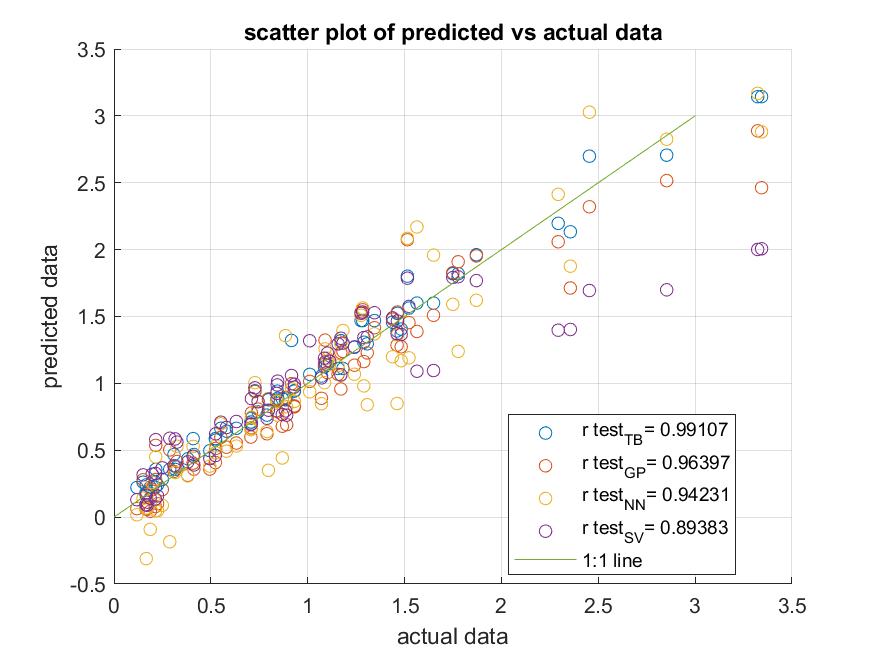
\includegraphics[width=1\textwidth]{new figures/disp_wCP2500.png}
    \end{minipage}
    \begin{minipage}{0.495\textwidth}
        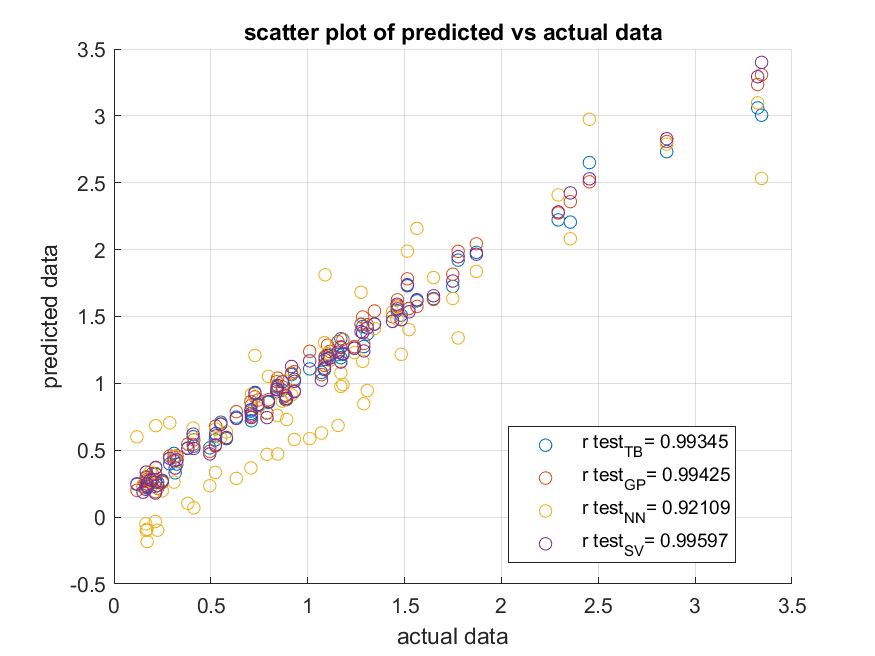
\includegraphics[width=1\textwidth]{new figures/disp_2500.png}
    \end{minipage}

    \begin{minipage}{0.495\textwidth}
        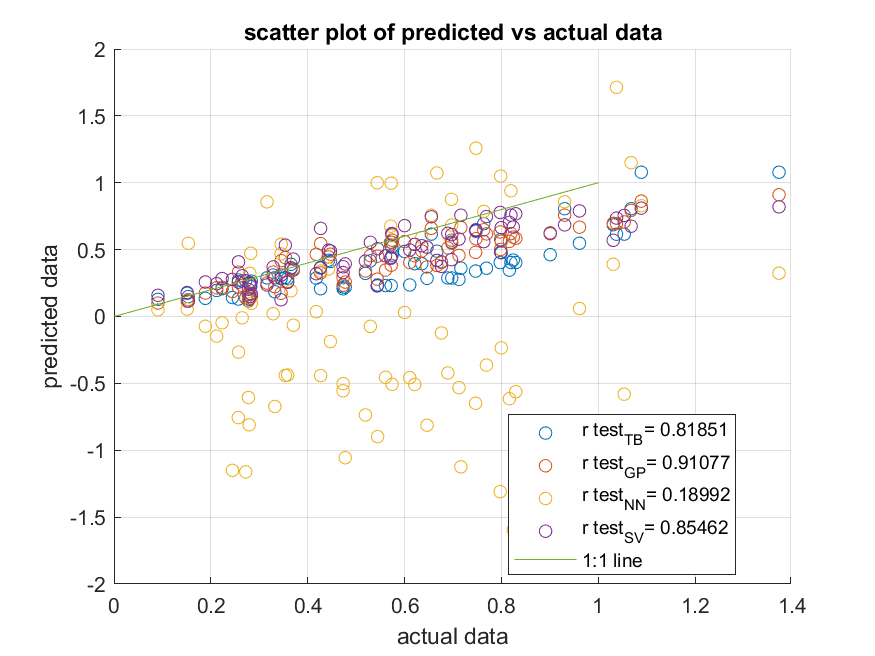
\includegraphics[width=1\textwidth]{new figures/cond_wCP2500.png}
    \end{minipage}
    \begin{minipage}{0.495\textwidth}
        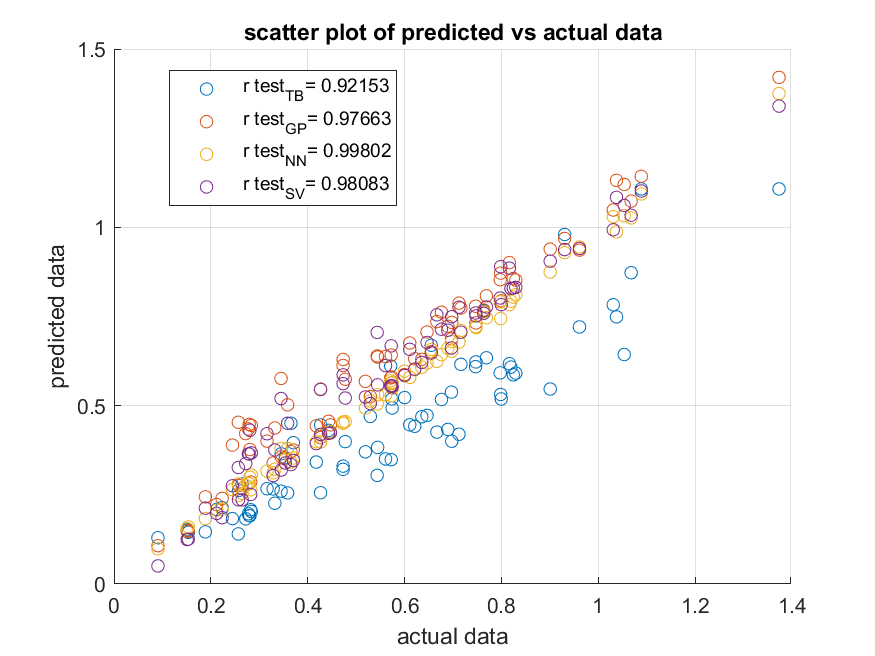
\includegraphics[width=1\textwidth]{new figures/cond_2500.png}
    \end{minipage}
    
    \begin{minipage}{0.495\textwidth}
        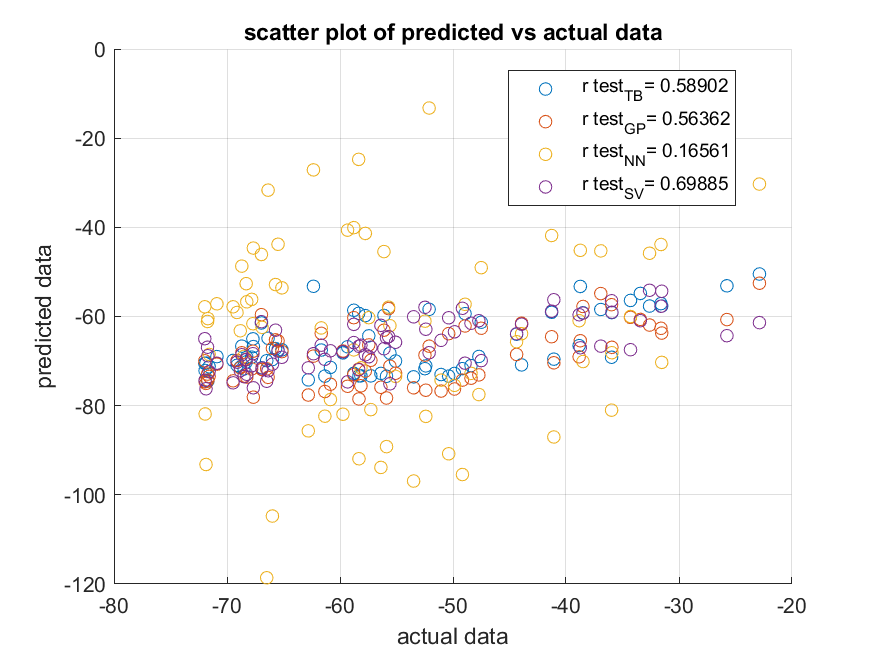
\includegraphics[width=1\textwidth]{new figures/phase_wCP2500.png}
    \end{minipage}
    \begin{minipage}{0.495\textwidth}
        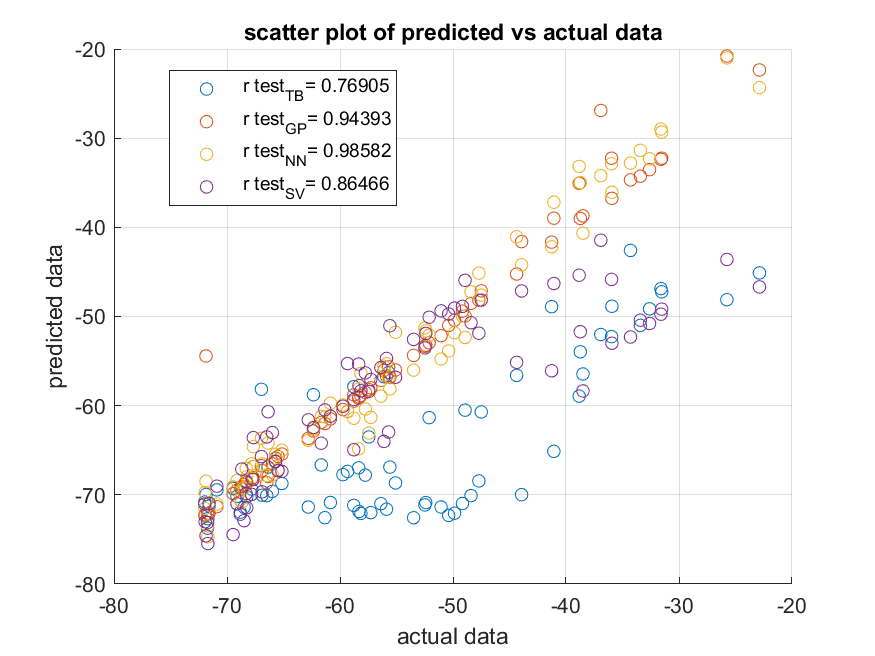
\includegraphics[width=1\textwidth]{new figures/phase_2500.png}
    \end{minipage}
    \caption{Extrapolation (BASED ON WHICH DATA SET?) of displacement current at 2.5 Torr with only control parameters (top left) vs. with total current as additional input (top right). Extrapolation of conduction current at 2.5 Torr with only control parameters (middle left) vs. with total and displacement current as additional inputs (middle right). Extrapolation of electrode phase at 2.5 Torr with only control parameters (bottom left) vs. with total and displacement current as additional inputs (bottom right) \textbf{font size needs to be fixed - some indication in the figures as to what is what... say pressure inside the figure and axis need better labels.}} 
\label{Fig:gap_SV,pressure_TB,species_TB}
\end{center}
\end{figure}

Interpolation and extrapolation were studied for phase-dependent parameters as well, specifically the phase difference, conduction and displacement current at the powered electrode. For interpolating these parameters at 1 and 2 Torr, Matrix 2 was used to predict and check fit against 90 observations at 1 and 2 Torr, with models trained from 804 observations at 0.5, 1.5 and 2.5 Torr. And for extrapolation at 2.5 and 0.5 Torrs, 594 observations were used for training and 300 observations for testing. When using only the control parameters as inputs, only the displacement current predictions were accurate with a correlation coefficient $>$0.95. Although displacement current depends on phase, having a low error bar could explain its prediction accuracy with only control parameters as inputs. Due to the slope of cosine being small at measured phases of the cycle [footnote], the variation in displacement current is less sensitive to change in phase resulting in a lower error bar. Nonetheless, prediction accuracy was seen to increase even more with fundamental current as an additional input. First harmonic current to the powered electrode was chosen as the additional input since it was ranked as the most important predictor by the random forest for both interpolation and extrapolation cases. Once the total and displacement currents were predicted accurately, high error bar parameters like conduction current and phase were predicted next. Prediction accuracy for high error bar parameters was less accurate with only the control parameters as inputs. But with total and displacement currents as additional inputs, machine learning models were able to predict conduction current and phase with great accuracy ($r>0.95$ for most cases). This is not surprising given the fact that conduction current or phase can be easily calculated in a single step [footnote] with the knowledge of total and conduction currents beforehand.
%The only exception to this was the first harmonic electrode phase at 1-2 Torr with a correlation coefficient of r=0.86.

%Nonetheless, the use of cumulative input parameters with the help of predictor importance ranking, eventually resulted in greater prediction accuracy for conduction currents as well as phases.


% Interpolation at 1 and 2 Torr for high error bar parameters: Use table 3 to Predict and check fit for measurements with high error bars (first harmonic phase dependent parameters) at 1 and 2 Torr (90 observation for testing) using all parameters having a good predicted fit (correlation coefficient >0.95) at 1 and 2 Torr as inputs along with the control parameters (804 observations for training).  Both conduction and displacement current and phase data were predicted with a correlation coefficient of () by at least one model. The best-performing models were (). Minimize the number of inputs other than the control parameters based on the ranking of input parameter importance given by the random forest model training.

% Extrapolation (with available data) for high error bar parameters at 2.5 Torr and at 0.5 Torr: Use table 3 to Predict and check fit for measurements with high error bars (first harmonic phase dependent parameters) at 2.5 Torr (300 observation for testing) using all parameters having a good predicted fit (correlation coefficient >0.95) at 2.5 Torr as inputs along with the control parameters (594 observations for training). All predicted low error bar parameters at 2.5 and 0.5 Torr with a good prediction accuracy were used as inputs at first but only the ones needed to give a prediction accuracy 0.98 or higher were kept based on the predictor importance ranking from the random forest model. Displacement current was predicted with a correlation coefficient of .. by the model.. Although displacement current was predicted accurately with only the control parameters and low error bar parameters as inputs, conduction current and phase data predictions were not as good. Nonetheless, conduction current prediction accuracy was increased substantially when displacement current was used as one of the inputs. Models were trained at lower pressures (0.5, 1, 1.5 and 2 Torrs). Similarly, predict and check fit at 0.5 Torr from models trained at higher pressures (1, 1.5, 2 and 2.5 Torr). Both conduction and displacement current and phase data were predicted with a correlation coefficient of () by at least one model. The best performing models were (). 


Once extrapolation accuracy was checked at the high and low end of the pressure range namely 2.5 and 0.5 Torrs, one can further extrapolate where experimental data is unavailable. Matrix 3 was used to predict fundamental voltage and currents at pressures greater than 2.5 Torr and smaller than 0.5 Torr. Predictions were made at 3.5 Torr with the model and inputs for that model giving the best fit at 2.5 Torr. The best model was trained for each respective parameter with all available data for that parameter at 0.5, 1.5, and 2.5 Torr. Similarly, predict them at 0.1 Torr using the best-fitting model at 0.5 Torr. \textcolor{red}{ Predictions for voltage and total current for pure argon, nitrogen, and oxygen at 3.5 and 0.1 Torr were then compared with predicted as well as experimental I-V curves at 0.5, 1, 2, and 2.5 Torrs.} ML predictions were found to be congruent with the experimental I-V trends at increasing/decreasing pressure.



\begin{figure}[ht!]
\begin{center}
    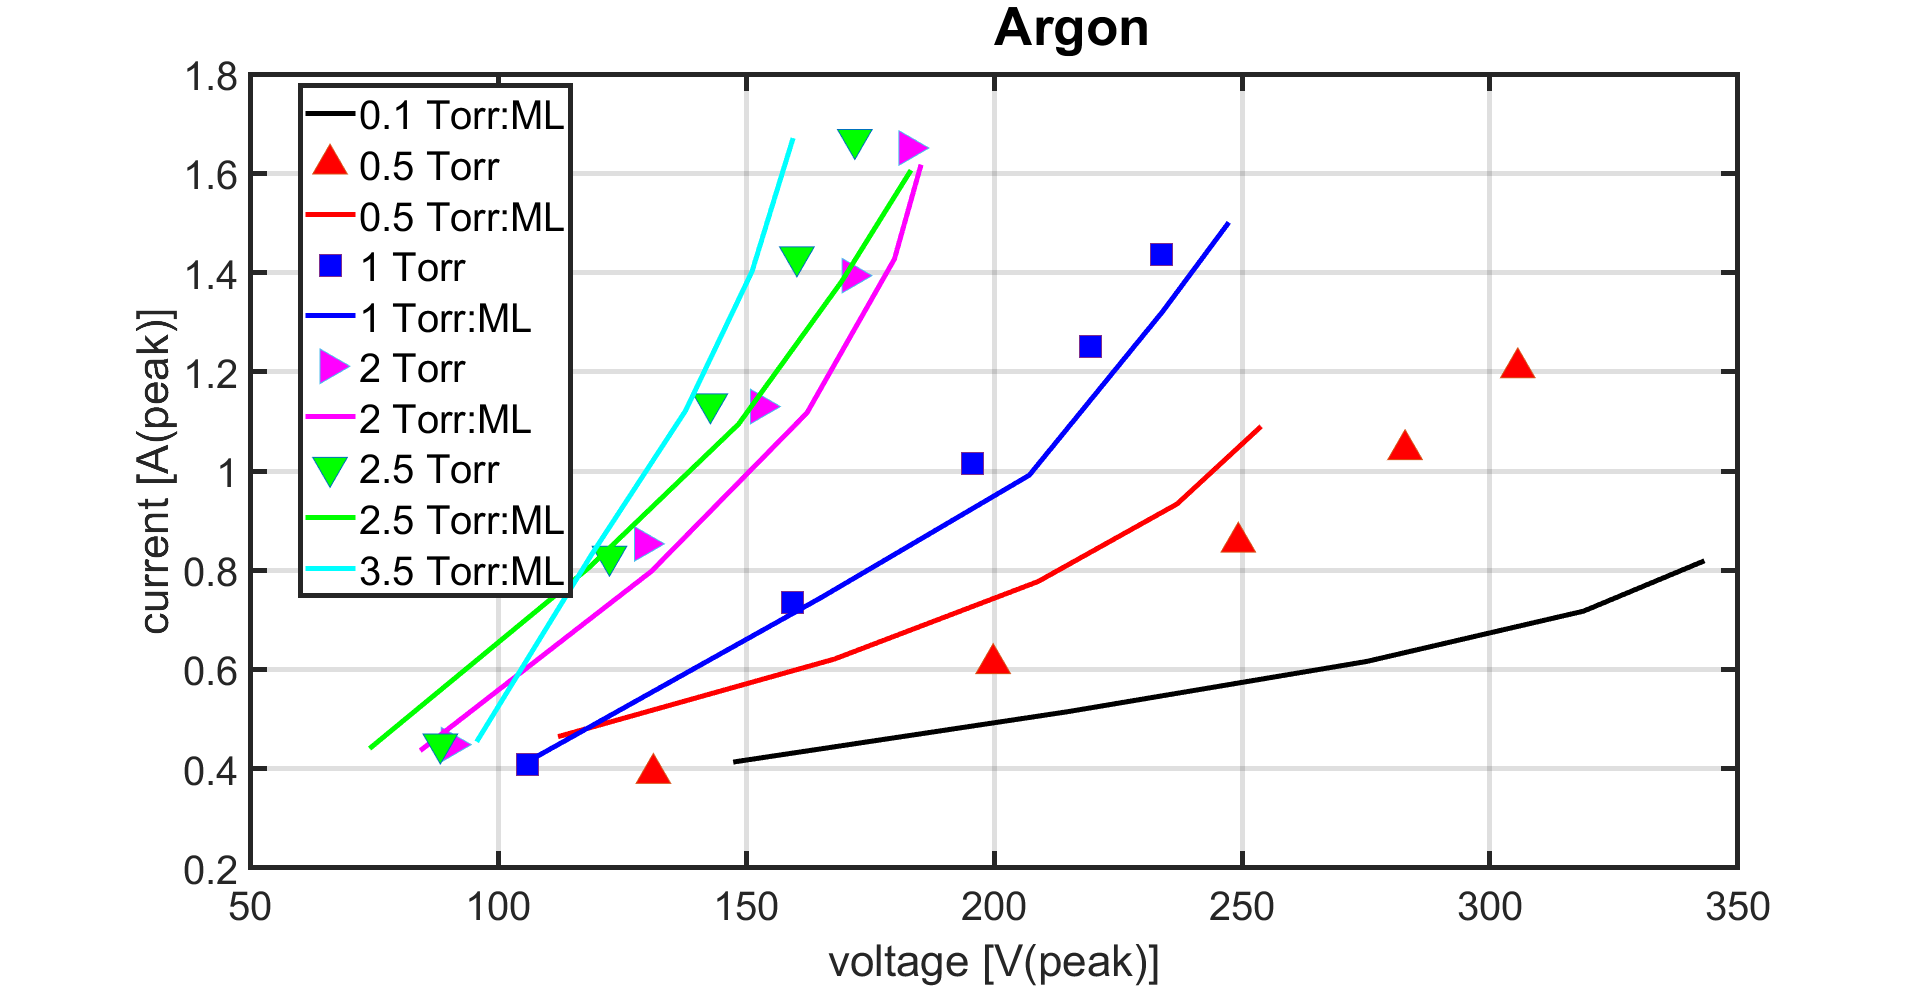
\includegraphics[width=.9\textwidth]{new figures/argon_real_pred.png}
    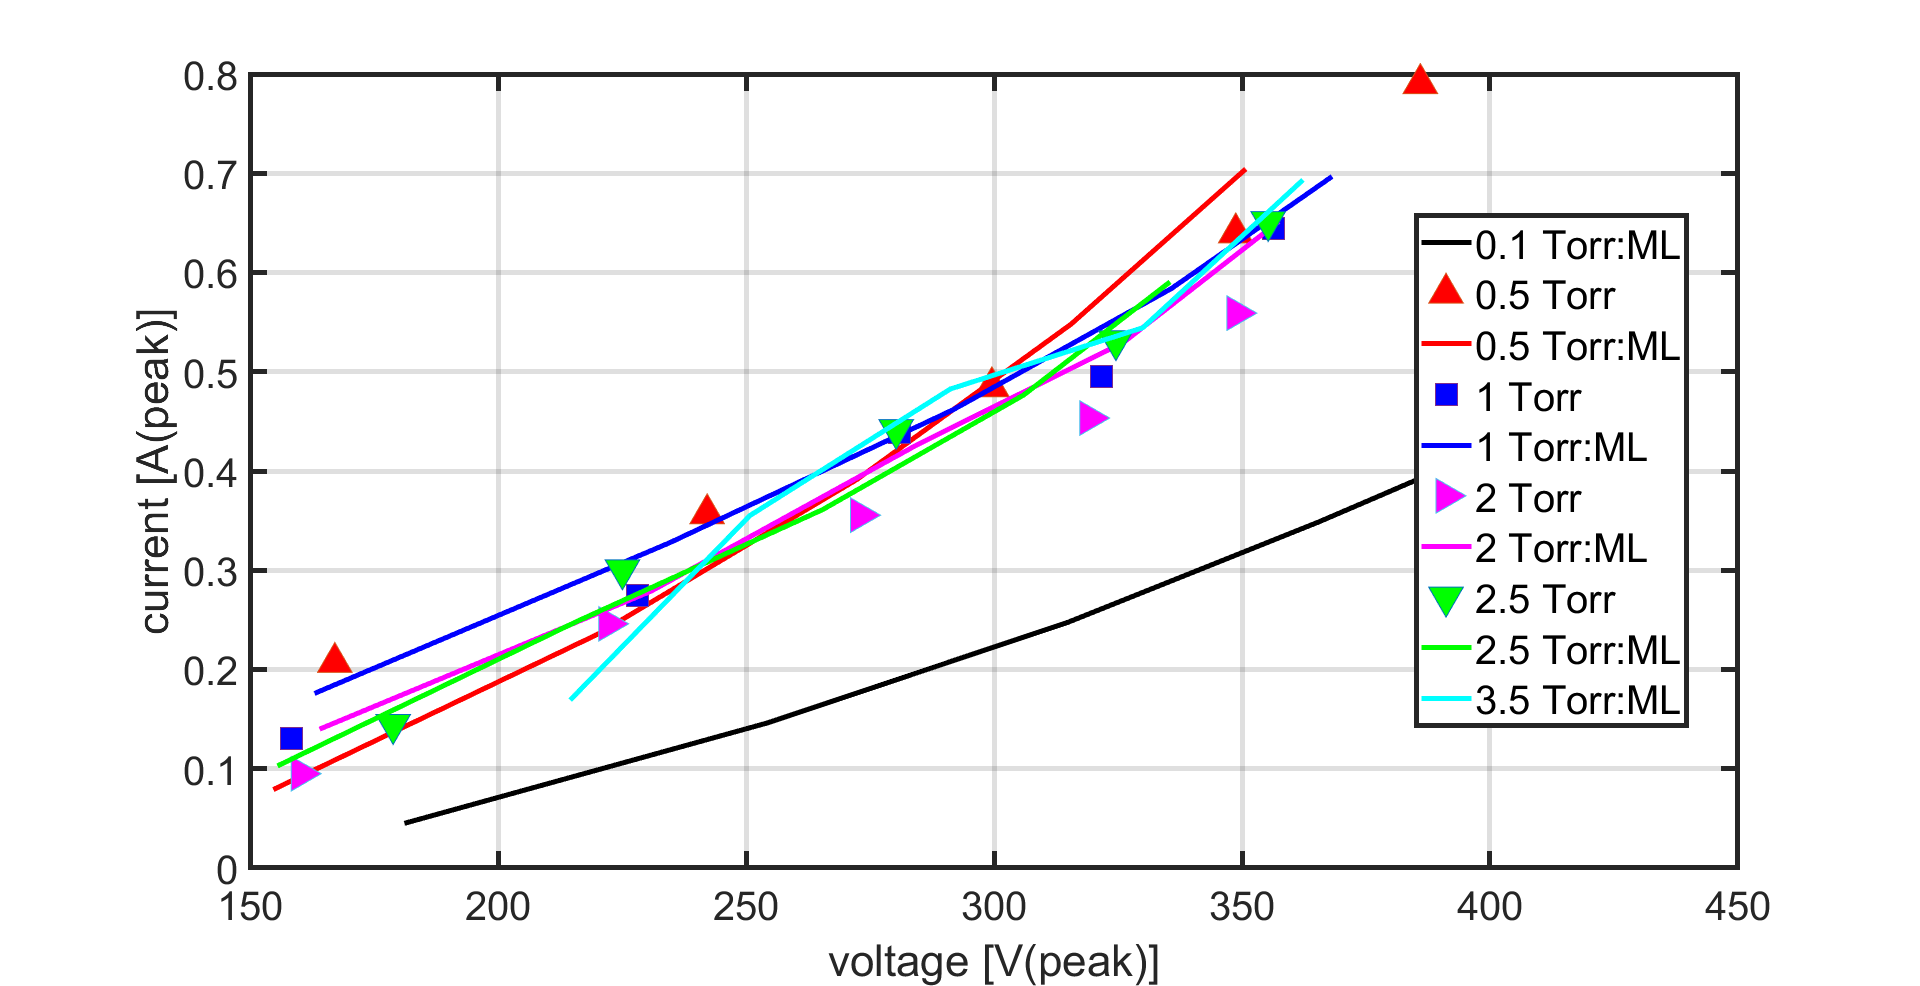
\includegraphics[width=.9\textwidth]{new figures/n2_real_pred.png}
    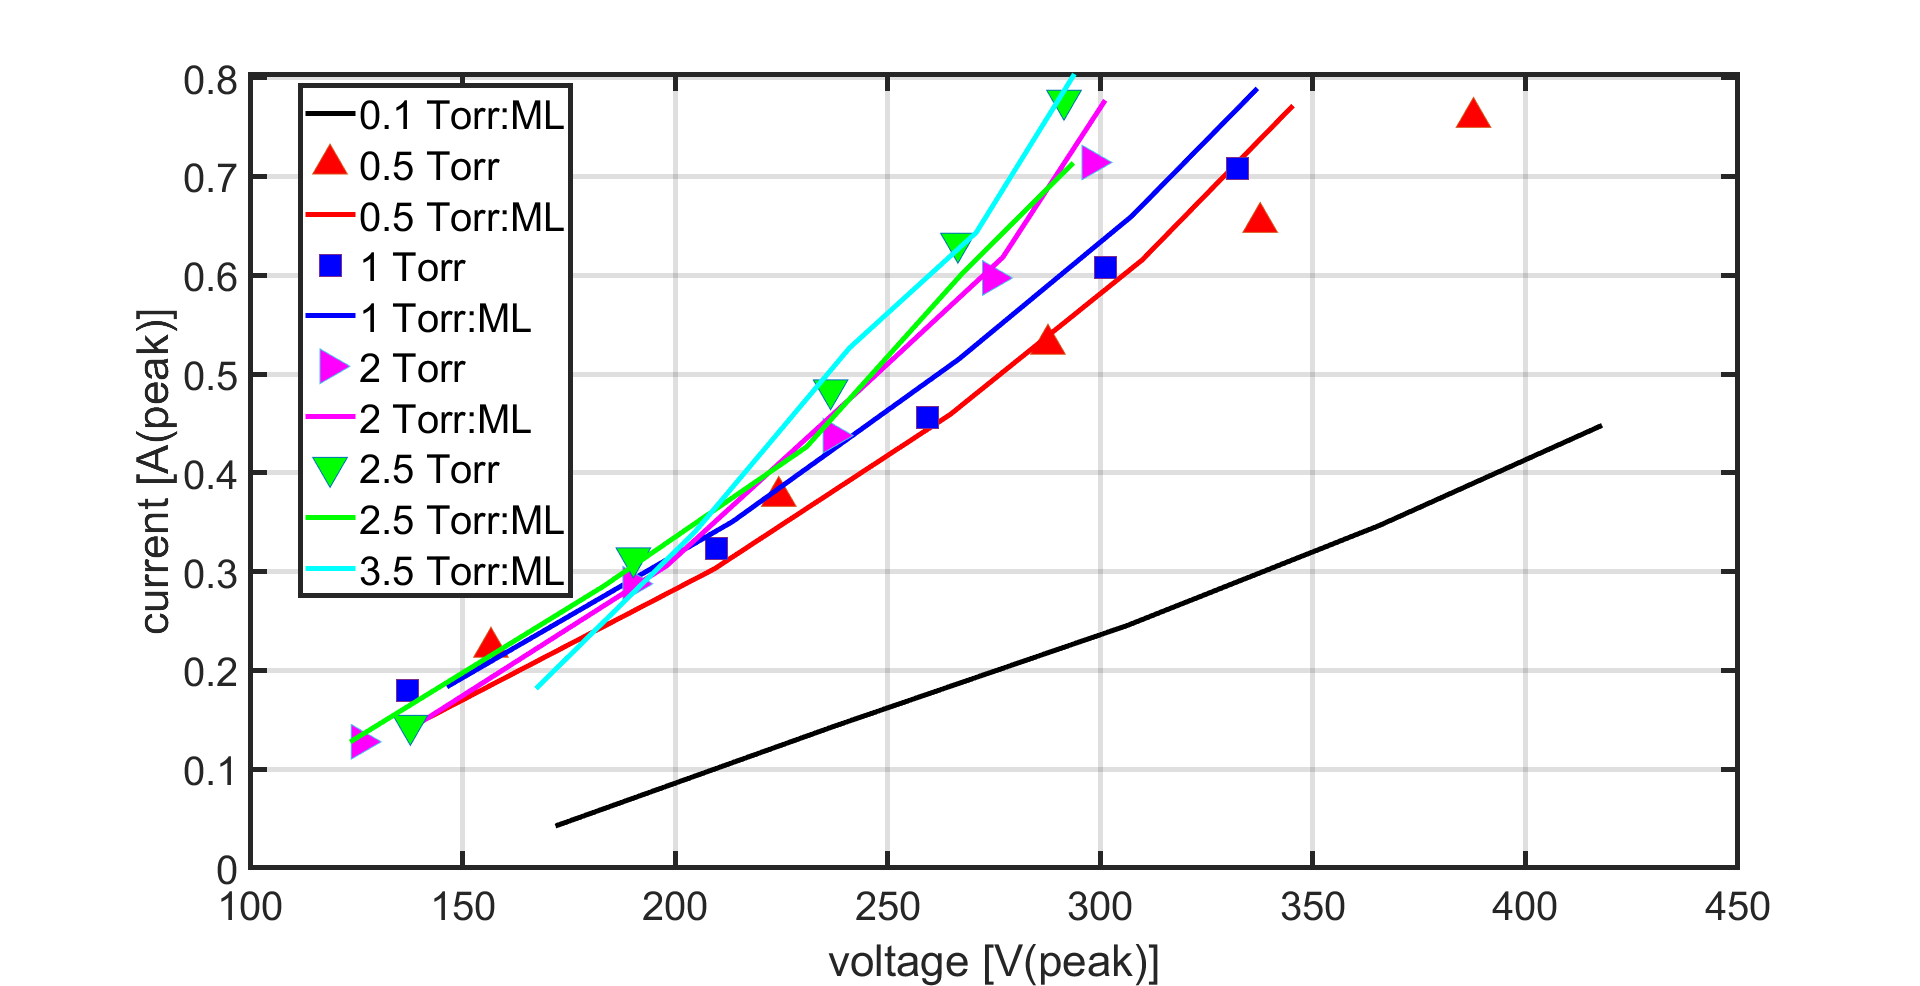
\includegraphics[width=.9\textwidth]{new figures/o2_real_pred.png}
\caption{Experimental vs. ML predictions. Extrapolations at 0.1 Torr and 0.3 Torr were made using matrix 3. For all other predictions matrix 1 was used.} 

\label{Fig:gap_SV,pressure_TB,species_TB}
\end{center}
\end{figure}



%Extrapolation (with NO available data) for low error bar parameters at higher (>2.5 Torr) and lower(<0.5 Torr) pressures: Choose the parameters with good fit (correlation coefficient >0.95) at 2.5 Torr and for each of those parameters use the model giving the best fit at 2.5 Torr. Train the model for each respective parameter with all available data for that parameter at 0.5, 1 , 1.5, 2 and 2.5 Torr and predict them at higher pressures (> 2.5 Torr) (75 x 10 matrix as output of the dataset) using matrix 2 (why?) with only the control parameters as inputs (291 x 6 matrix as input of the dataset). Similarly, predict them at lower pressures (<0.5 Torr) using the best fitting model at 0.5 Torr.

%Extrapolation (with NO available data) for high error bar parameters at higher (>2.5 Torr) and lower (<0.5 Torr) pressures: Use table 2 to predict high error bar parameters at higher pressures (>2.5 Torr), with the model and minimum number of inputs for that model giving the best fit at 2.5 Torr. Similarly, predict them at lower pressures (<0.5 Torr) using the best fitting model at 0.5 Torr. 


 

\begin{table}[]
    \centering
    
\begin{tabular}{|*{13}{c|}}  % repeats {c|} 18 times
\hline
\multicolumn{1}{|c}{parameter name} & \multicolumn{4}{|c}{interpolation (1-2 T)} & \multicolumn{4}{|c|}{extrapolation (0.5 T)} & \multicolumn{4}{|c|}{extrapolation (2.5 T)} \\ \hline

 & RF & NB & NN & SV & RF & NB & NN & SV & RF & NB & NN & SV \\ \hline
\multicolumn{13}{c}{Phase-independent parameters} \\
        \hline
        
$V_{DC}$ & 0.98 & 0.97 & 0.95 & 0.97 & 0.89 & 0.94 & 0.32 & 0.92 & 0.96 & 0.88 & 0.86 & 0.86\\ 
$V_{rf,1}$ &0.99 &0.998 &0.99 &0.998 &0.98 &0.99 &0.99 &0.96 &0.99 &0.99 &0.98 &0.97\\
$V_{rf,2}$ &0.99 &0.99 &0.96 &0.98 &0.93 &0.94 &0.95 &0.97 & 0.997&0.99 &0.98 &0.94\\
$V_{rf,3}$ &0.92 &0.92 &0.93 &0.94 &0.94 &0.94 &0.96 &0.97 &0.91 &0.88 &0.63 &0.82\\
$I_{rf,1}$ &0.99 &0.99 &0.99 &0.99 &0.95 &0.96 &0.86 &0.97 &0.995 &0.98 &0.97 &0.98\\
$I_{rf,2}$ &0.99 &0.99 &0.97 &0.99 &0.93 &0.94 &0.82 &0.96 &0.997 &0.98 &0.97 &0.96\\
$I_{rf,3}$ &0.93 &0.91 &0.92 &0.95 &0.93 &0.93 &0.91 &0.96 &0.91 &0.86 &0.76 &0.46\\
$I_{gnd,1}$ &0.98 &0.996 &0.993 &0.996 &0.93 &0.94 &0.94 &0.96 & 0.98& 0.99& 0.96&0.96\\
$I_{gnd,2}$ &0.98 &0.96 &0.92 &0.95 &0.84 &0.84 &0.79 &0.81 &0.98 &0.97 &0.37 &0.83\\
$I_{gnd,3}$ & 0.9&0.86 &0.82 &0.79 &0.68 &0.76 &0.78 &0.82 & 0.92&0.95 &0.38 &0.84\\
 \hline
 
\end{tabular}

 \caption{Prediction accuracy (r-coefficient) for phase-independent parameters (using Matrix 1) with control parameters as inputs}
 
\end{table}



\begin{table}[]
    \centering
    
\begin{tabular}{|*{13}{c|}}  % repeats {c|} 18 times
\hline
\multicolumn{1}{|c}{parameter name} & \multicolumn{4}{|c}{interpolation (1-2 T)} & \multicolumn{4}{|c|}{extrapolation (0.5 T)} & \multicolumn{4}{|c|}{extrapolation (2.5 T)} \\ \hline

 & RF & NB & NN & SV & RF & NB & NN & SV & RF & NB & NN & SV \\ \hline
\multicolumn{13}{c}{First harmonic phase-dependent parameters} \\
        \hline

$I_{cond,1}$ & 0.67&0.67 &0.65 &0.69 & 0.59&0.81 &0.05 &0.84 &0.82 &0.91 &0.19 &0.85\\ 
$I_{disp,1}$ &0.99 &0.96 &0.99 &0.92 &0.95 &0.96 &0.88 &0.97 &0.99 &0.96 &0.94 &0.89\\
$R_{1}$ &0.92 &0.88 &0.84 &0.77 &0.84 &0.85 &0.49 &0.83 &0.93 &0.92 &0.29 &0.84\\
$X_{1}$ &0.76 &0.8 &0.74 &0.89 &0.88 &0.85 &0.37 &0.92 &0.78 &0.73 &0.48 &0.76\\
$P_{1,e}$ &0.73 &0.72 &0.71 &0.84 & 0.82 &0.96 &0.42 &0.95&0.81 &0.92 &0.65 &0.93\\
$P_{1,p}$ &0.86 & 0.85&0.78 & 0.94& 0.91 &0.98 &0.5 &0.96 &0.9 &0.94 &0.1 &0.95\\
$\nu_{1,e}$ &0.36 &0.29 &0.29 &0.46 &0.374 &0.57 &0.21 &0.59 & 0.59&0.56 &0.17 &0.7\\
$\nu_{1,p}$ & 0.69&0.64 &0.61 &0.7 & 0.35&0.32 &$<0$ &0.32 &0.86 &0.76 &0.61 &0.63\\
 \hline
\multicolumn{13}{c}{2nd harmonic phase-dependent parameters} \\
        \hline
$I_{cond,2}$ &0.91 &0.98 &0.94 &0.78 &0.9 &0.94 &0.93 &0.92 &0.99 &0.97 &0.91 &0.88\\ 
$I_{disp,2}$ &0.93 &0.99 &0.98 & 0.82&0.92 &0.94 &0.88 &0.97 &0.99 &0.94 &0.75 &0.94\\
$R_{2}$ &0.33 &0.38 &0.35 &0.32 &0.32 &0.35 &0.11 &0.36 &0.56 &0.45 &0.10 &$<0$\\
$X_{2}$ &$<0$ &$<0$ &$<0$ & $<0$&0.63 &0.46 &$<0$ &0.47 &0.24 &$<0$ &$<0$ &0.55\\
$P_{2,e}$ &0.92 &0.99 &0.95 &0.99 & 0.85&0.9 &0.8 &0.86 & 0.99& 0.79 &0.85 &0.96\\
$P_{2,p}$ &0.71 &0.66 &0.77 &0.52 &0.72 &0.81 &0.66 &0.74 &0.88 &0.7 &0.82 &0.44\\
$\nu_{2,e}$ &0.38 &0.42 &0.31 &0.42 &0.26 &0.24 &0.05 &0.31 &0.69 &0.44 &$<0$ &0.41\\
$\nu_{2,p}$ &0.28 &0.31 &0.05 &0.33 &0.34 &0.16 &0.18 &0.28 &0.21 & 0.48 &0.14 & 0.07\\
 \hline
 \multicolumn{13}{c}{3rd harmonic phase-dependent parameters} \\
        \hline
$I_{cond,3}$ &0.75 &0.80 &0.76 &0.76 & 0.83& 0.91 &0.53 &0.90 &0.73 &0.62 &0.17 &$<0$\\ 
$I_{disp,3}$ &0.85 &0.86 &0.92 &0.87 &0.93 &0.94 &0.83 &0.95 &0.90 &0.78 &0.55 &0.82\\
$R_{3}$ &0.05 &$<0$ &0.01 &0.02 &0.25 &0.13 &0.11 &0.16 &0.12 &0.55 & $<0$&0.41\\
$X_{3}$ &0.4 &0.44 &0.4 &0.53 &0.41 &0.27 &0.02 &0.37 & 0.37& 0.33& 0.09&0.47\\
$P_{3,e}$ &0.75 &0.76 &0.51 &0.69 & 0.82& 0.83&0.73 &0.89 &0.77 &0.01 &0.08 &0.75\\
$P_{3,p}$ &0.6 &0.58 & 0.54&0.51 &0.65 &0.83 &0.17 &0.8 &0.62 &$<0$ &$<0$ &0.65\\
$\nu_{3,e}$ &0.08 &0.04 &0.02 & $\approx 0$ &0.25 &0.17 &$<0$ &0.17 & 0.15&0.2 &$<0$ &0.39\\
$\nu_{3,p}$ &0.17 &0.15 &0.13 &0.30 &0.25 &0.29 &$<0$ &0.32 &0.11 &0.24 & $<0$&0.46\\
 \hline
 
\end{tabular}

 \caption{Prediction accuracy (r-coefficient) for phase-dependent parameters (using Matrix 2) with control parameters as inputs}
 
\end{table}

%\subsection{interpolation accuracy at 1 and 2 Torr}
%\subsection{extrapolation accuracy testing for magnitude and phase at 2.5Torr }
%\subsection{prediction using control parameters}
%\subsection{increasing prediction accuracy with added features}
%\subsection{predicting phase and phase dependent variables}
%\subsection{extrapolation at pressures beyond 2.5}

\section{Classification of control parameters}\label{Sect:Classification}


\begin{figure}[ht!]
\begin{center}
\begin{minipage}{0.5\textwidth}
    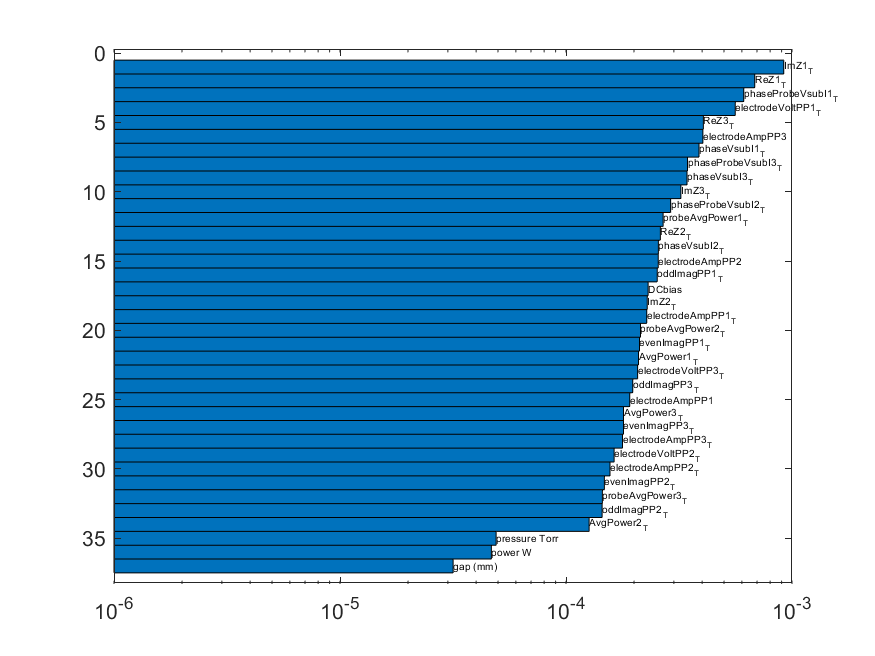
\includegraphics[width=1\textwidth]{input-importance-curvature-testSpecies.png}
\end{minipage}
\begin{minipage}{0.5\textwidth}
    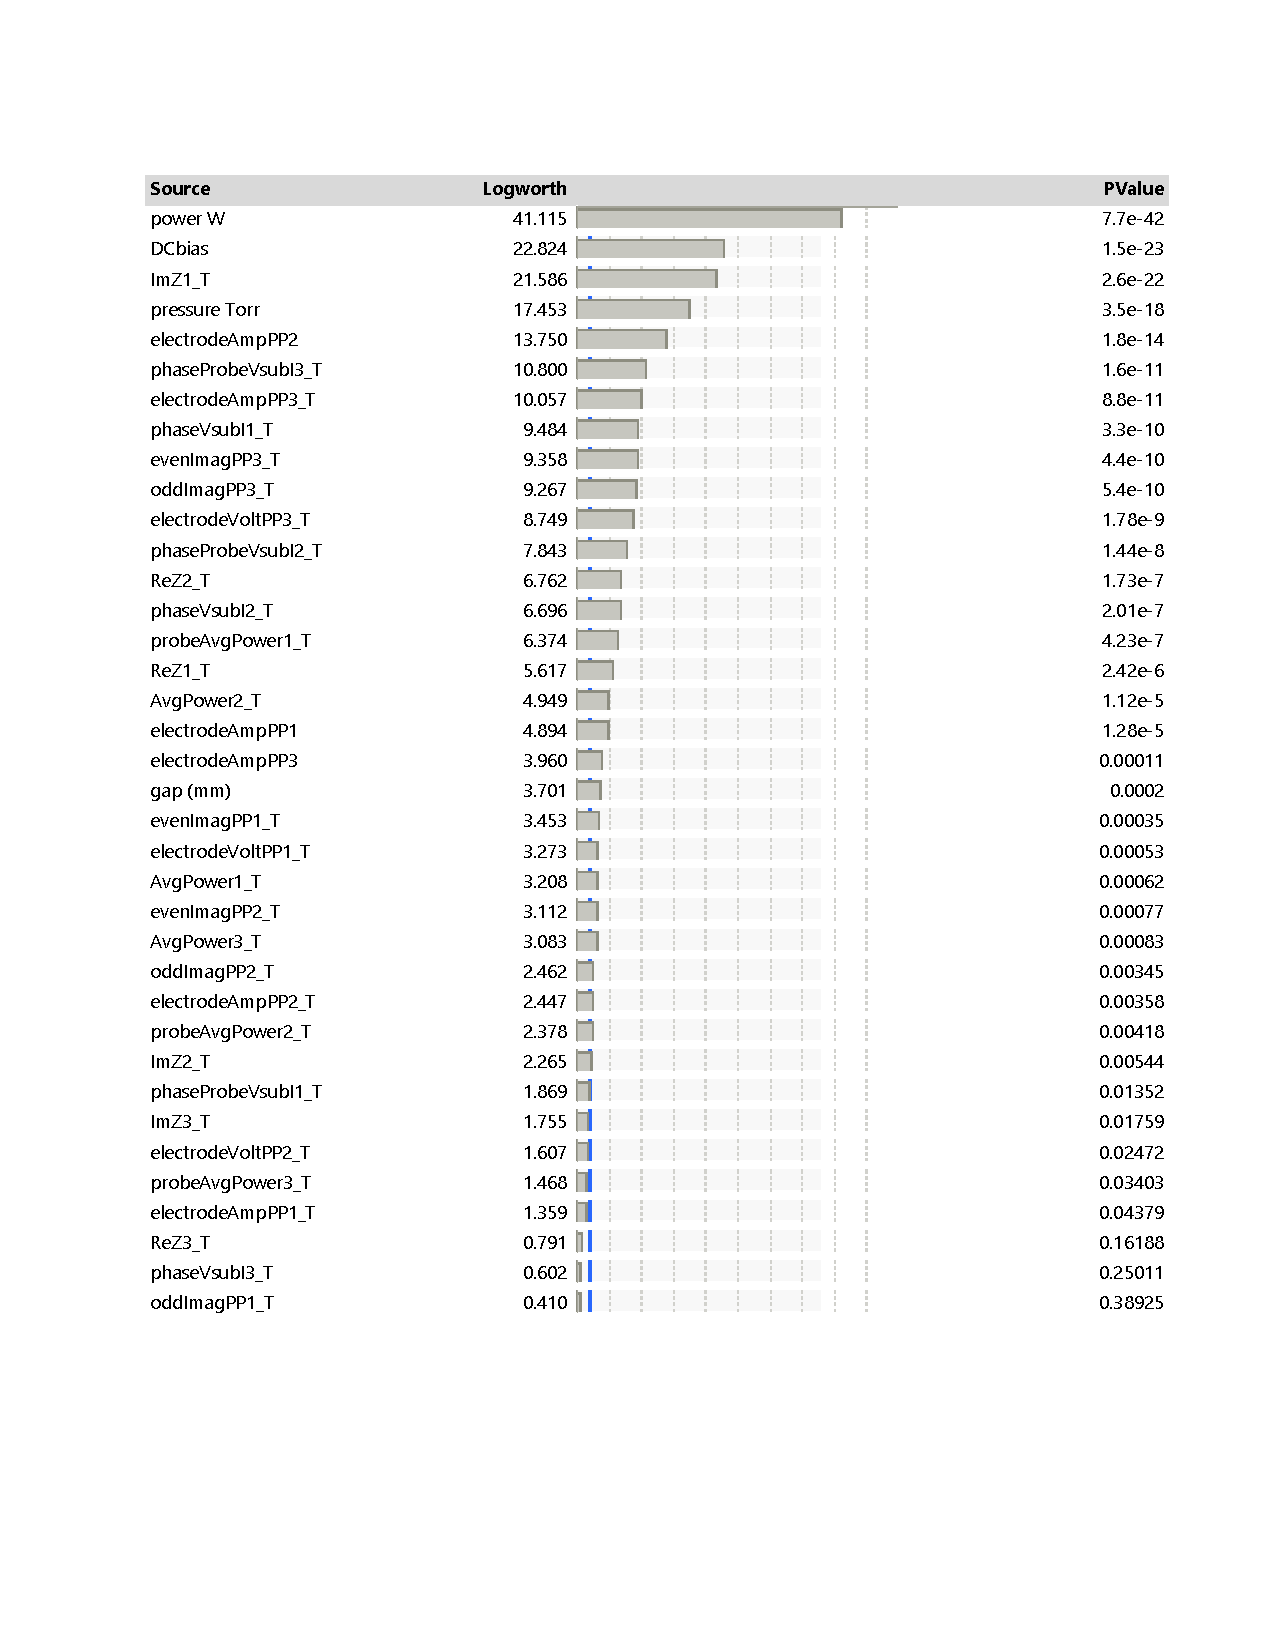
\includegraphics[width=1\textwidth]{jmpSpecies.pdf}
\end{minipage}

\caption{Predictor importance ranking for feed gas by random forest (top), p-value ranking of input parameters for least square fitting feed gas  (bottom) } 

\label{Fig:gap_SV,pressure_TB,species_TB}
\end{center}
\end{figure}

\begin{figure}[ht!]
\begin{center}
\begin{minipage}{0.5\textwidth}
    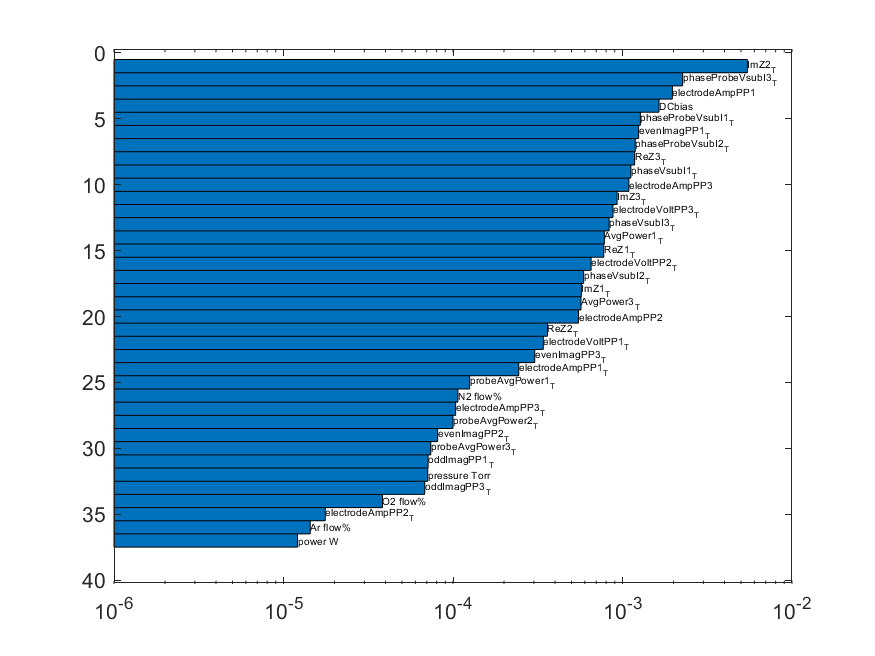
\includegraphics[width=1\textwidth]{input-importance-curvature-testGap.png}
\end{minipage}
\begin{minipage}{0.5\textwidth}
    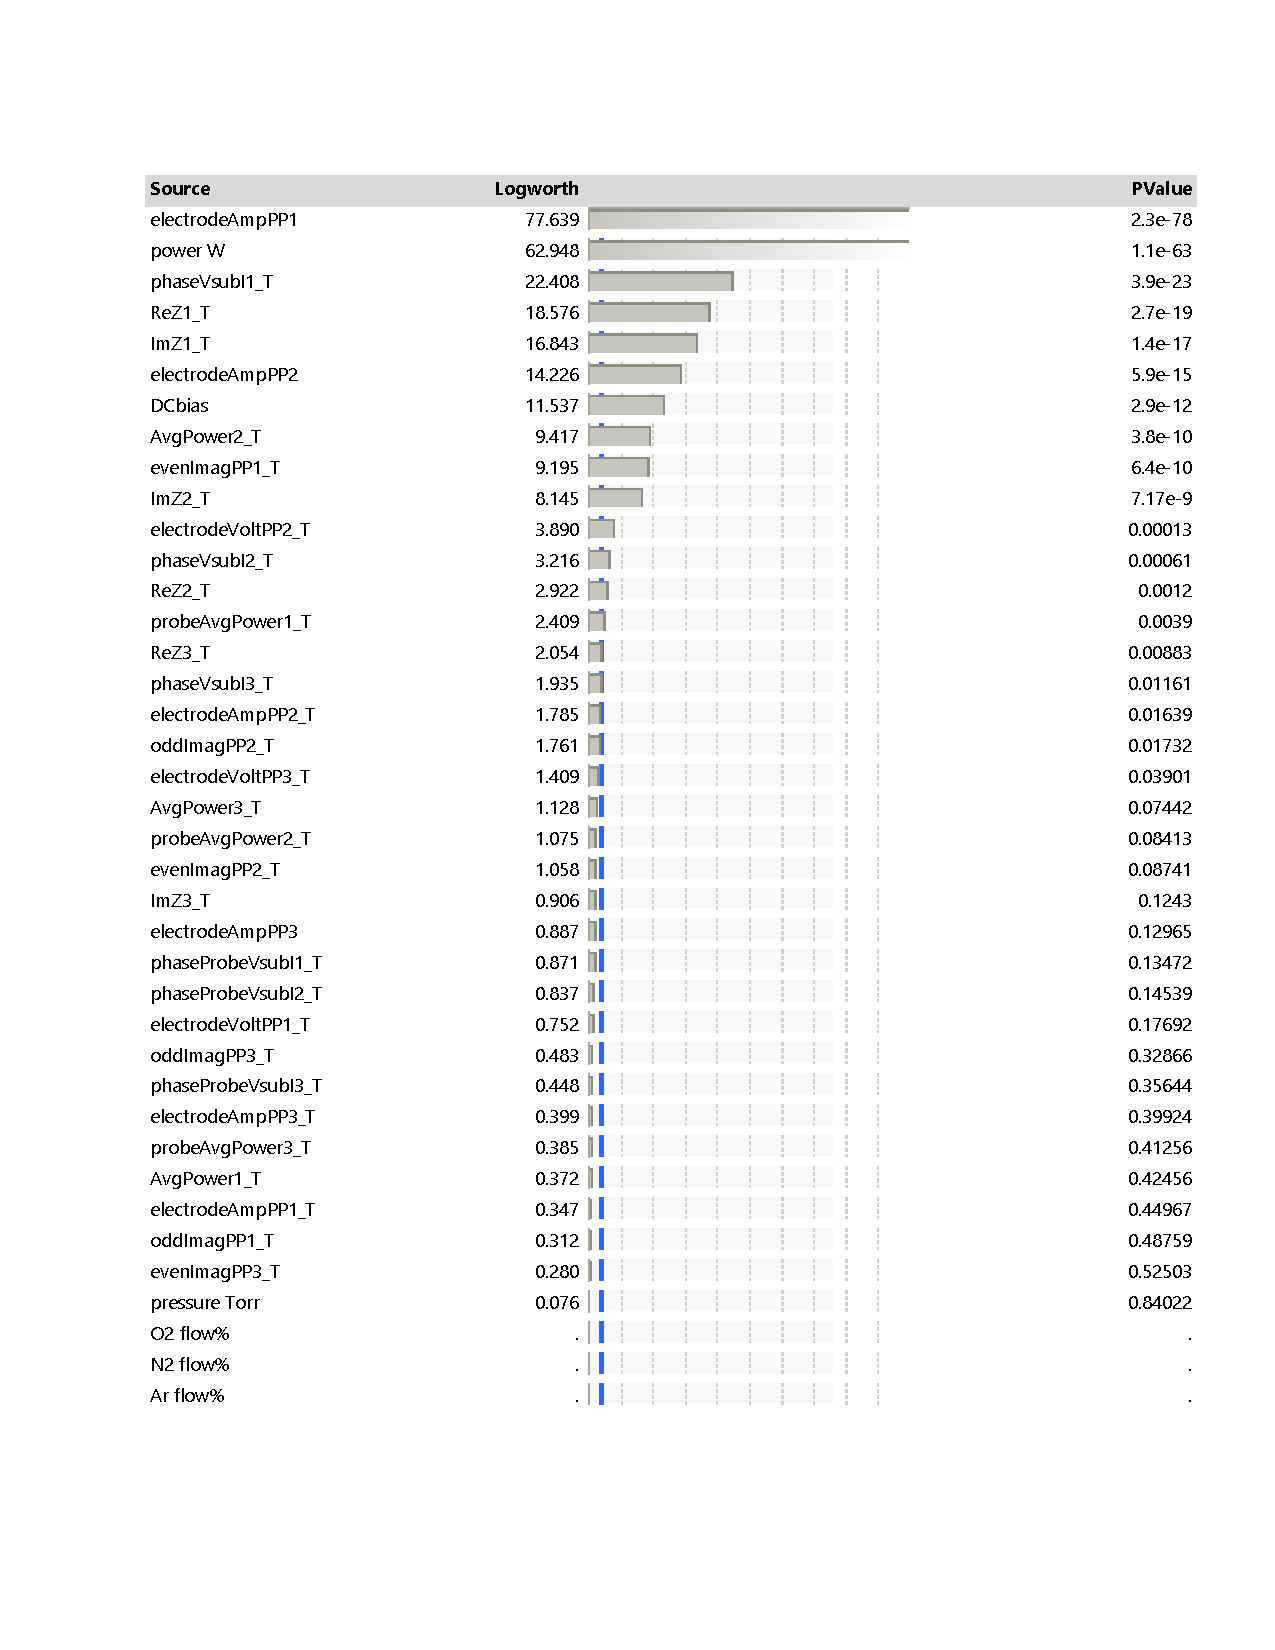
\includegraphics[width=1\textwidth]{jmpGap.pdf}
\end{minipage}

\caption{Predictor importance ranking for electrode gap by random forest (top),  p-value ranking of input parameters for least square fitting electrode gap  (bottom) } 

\label{Fig:gap_SV,pressure_TB,species_TB}
\end{center}
\end{figure}


\begin{figure}[ht!]
\begin{center}
\begin{minipage}{0.5\textwidth}
    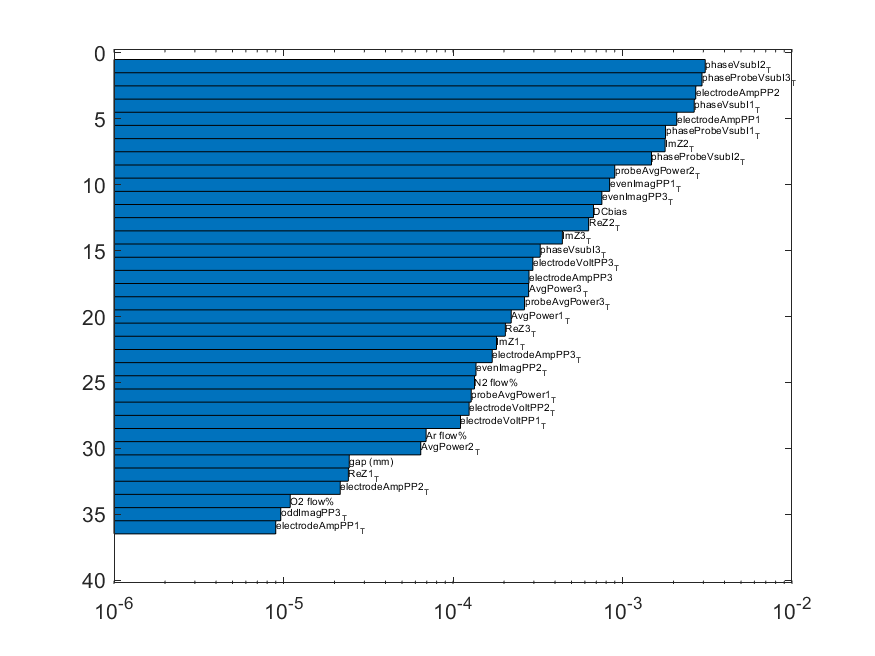
\includegraphics[width=1\textwidth]{input-importance-curvature-testPressure.png}
\end{minipage}
\begin{minipage}{0.5\textwidth}
    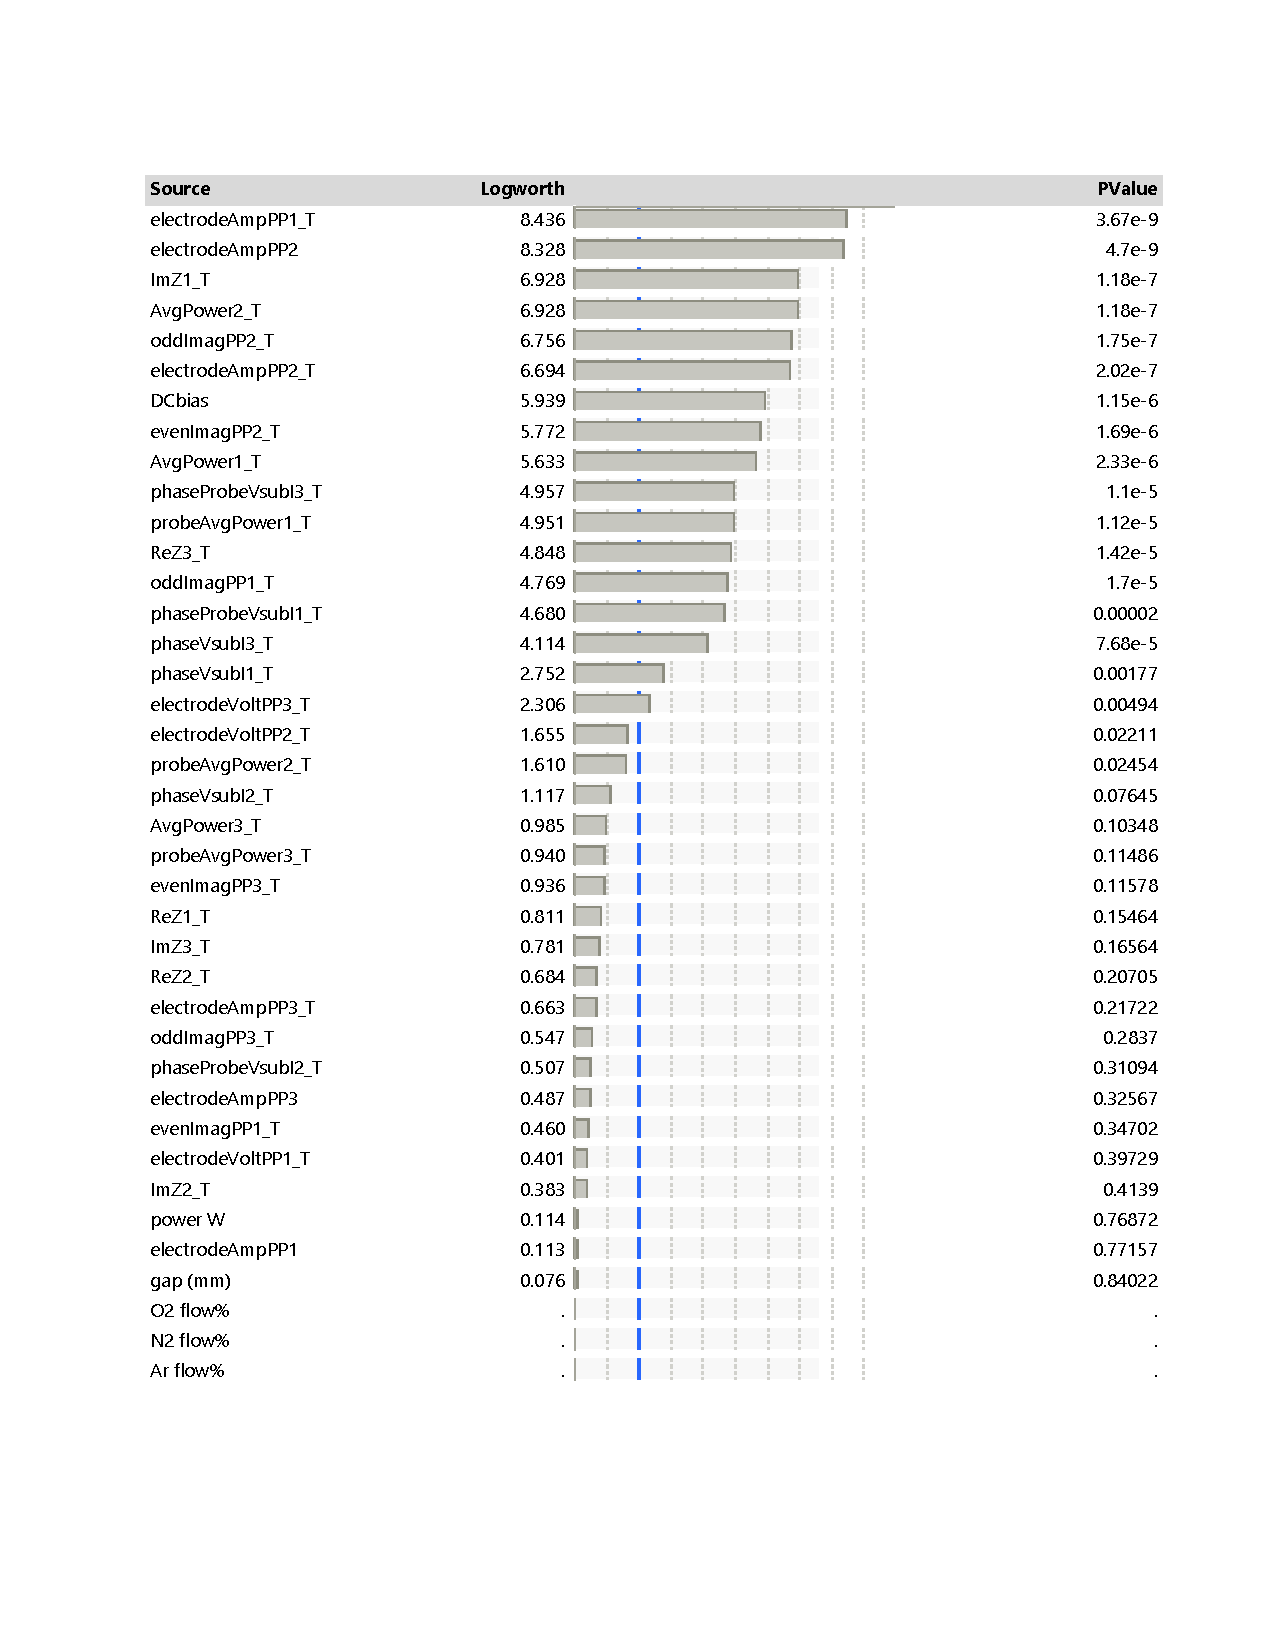
\includegraphics[width=1\textwidth]{jmpPressure.pdf}
\end{minipage}

\caption{Predictor importance ranking for pressure by random forest (top), p-value ranking of input parameters for least square fitting pressure (bottom) } 

\label{Fig:gap_SV,pressure_TB,species_TB}
\end{center}
\end{figure}
Five different classification models were used for comparison for the supervised classification studies namely 1) a neural network model for pattern recognition (patternnet), 2) an ensemble tree model (fitcensemble), 3) a naïve bayes model (fitcnb), 4) a support vector model (fitcsvm) and, 5) a linear discriminant analysis (fitcdscr). These models were used to classify the data by three of the four control parameters namely the operating pressure, gap, and the gas content of the plasma. For classification studies, Matrix 2 was used to check prediction accuracy for a given control parameter using all 34 parameters as well as the remaining control parameters as inputs. The models were randomly trained on 80\% of all 894 observations and tested on the rest 20\% of the observations. The models were optimized during the training. The neural network model was optimized by cross-validating 15\% of the data and testing 15\% of the data while the rest was used for training. The number of hidden layers was 30. On the other hand, the shallow models were optimized by 'automatic' tuning of various parameters that control the learning process i.e the hyperparameters [reference] of the respective models. Moreover, predictors were ranked based on their relative importance using the "out of bag delta error" object under the ensemble tree model. For a given control parameter, a least square fitting optimization was also done with JMP using all remaining parameters as predictors [refer to variable list]. Predictor parameters were ranked in descending order of their p-values. The predictor importance ranking of the random forest model was compared to the p-value ranking for the combined least square fit for the respective control parameter with JMP. \textbf{write comparative analysis of the two rankings}

Both ML and JMP predictions yielded great accuracy [ref. figure]. The p-values between the predictions obtained by a least-square fit and actual values were less than 0.0001 for each classification [refer to table]. On the other hand, all ML models were able to predict the class accurately almost all the time. The Area Under Curve (AUC) [ref] of the Receiver Operating Characteristics (ROC) plots [ref] for each value of all the control parameters was very close to 1. "AUC is the probability that a classifier will be more confident that a randomly chosen positive example is actually positive than that a randomly chosen negative example is positive." Moreover, the effect of principal component analysis (PCA) was also studied for all the classification models. For the PCA studies, components with 99\% cumulative variances were kept. The application of PCA decreased the prediction accuracy substantially. This could be due to the nonlinearity of the I-V dataset.

\textbf{report AUC values as a table and copy confusion matrices from MATLAB for only the best model. Describe the name of the best performing model in text. define AUC in text. Make another table with p-value and correct percent accuracy side by side?}

\begin{figure}[ht!]
\begin{center}
\begin{minipage}{0.495\textwidth}
    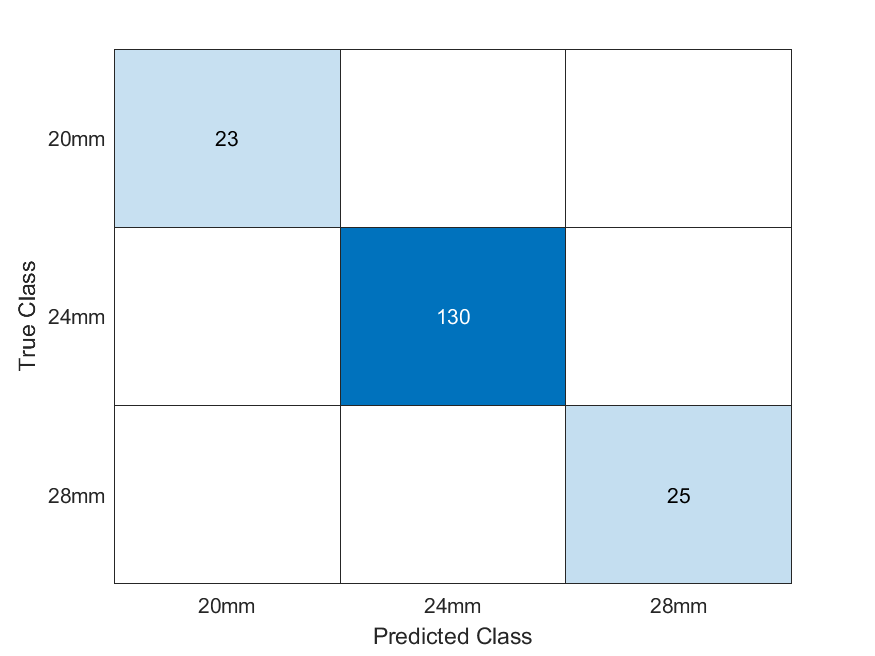
\includegraphics[width=1\textwidth]{ConfusionMatrix_SV.png}
\end{minipage}
\begin{minipage}{0.495\textwidth}
    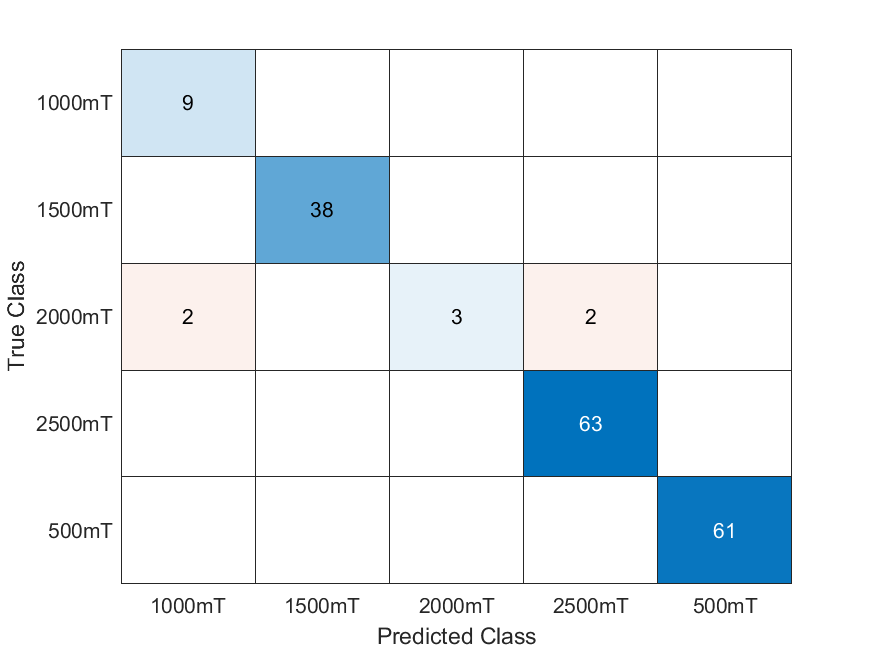
\includegraphics[width=1\textwidth]{ConfusionMatrixTB.png}
\end{minipage}

 \begin{minipage}{0.495\textwidth}
    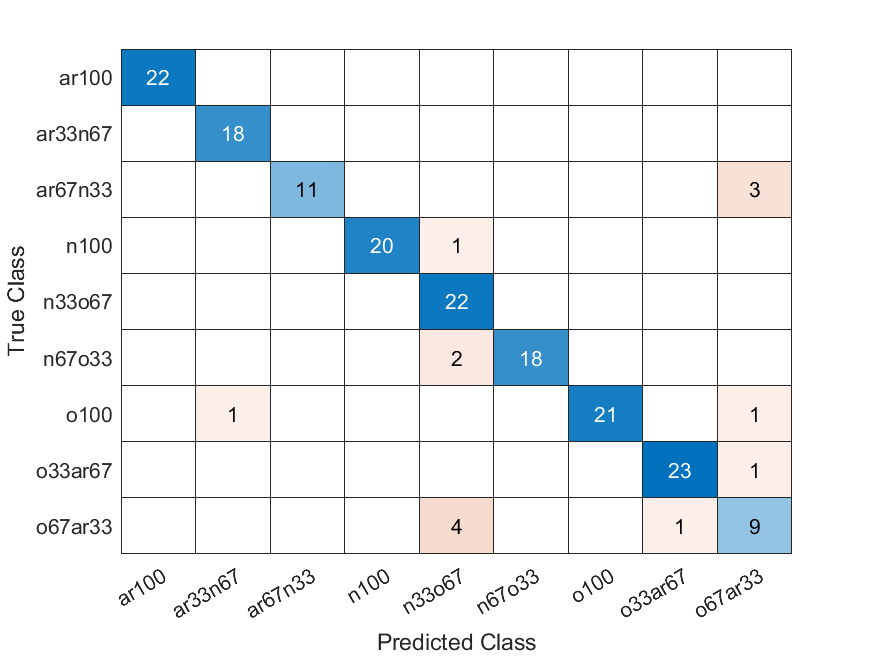
\includegraphics[width=1\textwidth]{ConfusionMatrixTB2.png}
\end{minipage}
\caption{Confusion matrix for Gap (SV) (top left), pressure (TB) (top right), and species (TB) (bottom) } 

\label{Fig:gap_SV,pressure_TB,species_TB}
\end{center}
\end{figure}


\section{Conclusions and future work}\label{Sect:Conclusions}

In this article, we have used statistical as well as machine learning predictions to analyze and organize I-V data in a moderate pressure capacively coupled plasma (CCP). We have demonstrated that deep neural network (DNN) as well as shallow machine learning models can be a useful tool for extrapolating data even with a high error bar at a transitional regime. Specifically, phase data with high error bars can be predicted with great accuracy which can be used to automatically tune matching networks. Classification of control parameters is another possible application of these models given a large set of measured data is available. The models were able to identify the gas ratio in the feed gas as well as correctly identify the operating pressure and electrode gap in almost all the cases. The importance of the predictors was ranked for these classification predictions. While input parameter importance can give some insight into the physics, comparison with physics-informed models is necessary. In future works, Physics-informed learning, such as physics-informed neural networks (PINNs) [ref-nature paper] will be explored on the mGEC moderate pressure database. Physics-informed learnings, can integrate domain knowledge and physical laws into ML models, improving their interpretability and accuracy, even with imperfect data. The availability of data and complexity of the system influence the specific data-driven approach for predictive modelling.



\section{Acknowledgements}
This work was supported by a generous donation from Applied Materials Inc.

\printbibliography %Prints bibliography


\end{document}

